\chapter{Charged Lepton Flavor Violation}
\textit{This chapter offers a concise overview of the fundamental theoretical and experimental components essential to understand the objectives of the Mu2e experiment at Fermilab and the work conducted for this Thesis. The introduction to the Standard Model and certain extensions serves to justify the investigation of Charged Lepton Flavor Violation (CLFV), since it would be a clear signal of new physics beyond the current theories. Fundamental bibliography for this chapter can be found in Ref. \cite{Bernstein_2013} and \cite{clfv_signorelli}.}
\section{Theoretical Introduction}
\subsection{The Standard Model}
The Standard Model provides an excellent description of elementary particles and their interactions. It describes three out of four the fundamental forces known to this day: electromagnetism interaction, weak interaction and strong interaction. This theory is based on the gauge symmetry group $U(1)_Y \times SU(2)_L \times SU(3)_C$. The first two terms describe the electroweak interaction, $Y$ indicates the hypercharge and $L$ refers to the fact that this acts only on the left handed components of the fields. The last term describes the strong interaction and $C$ indicates the color charge.
The Standard Model contains 25 elementary fields, shown in Fig. \ref{fig:sm}.

\begin{figure}[!h]
\centering
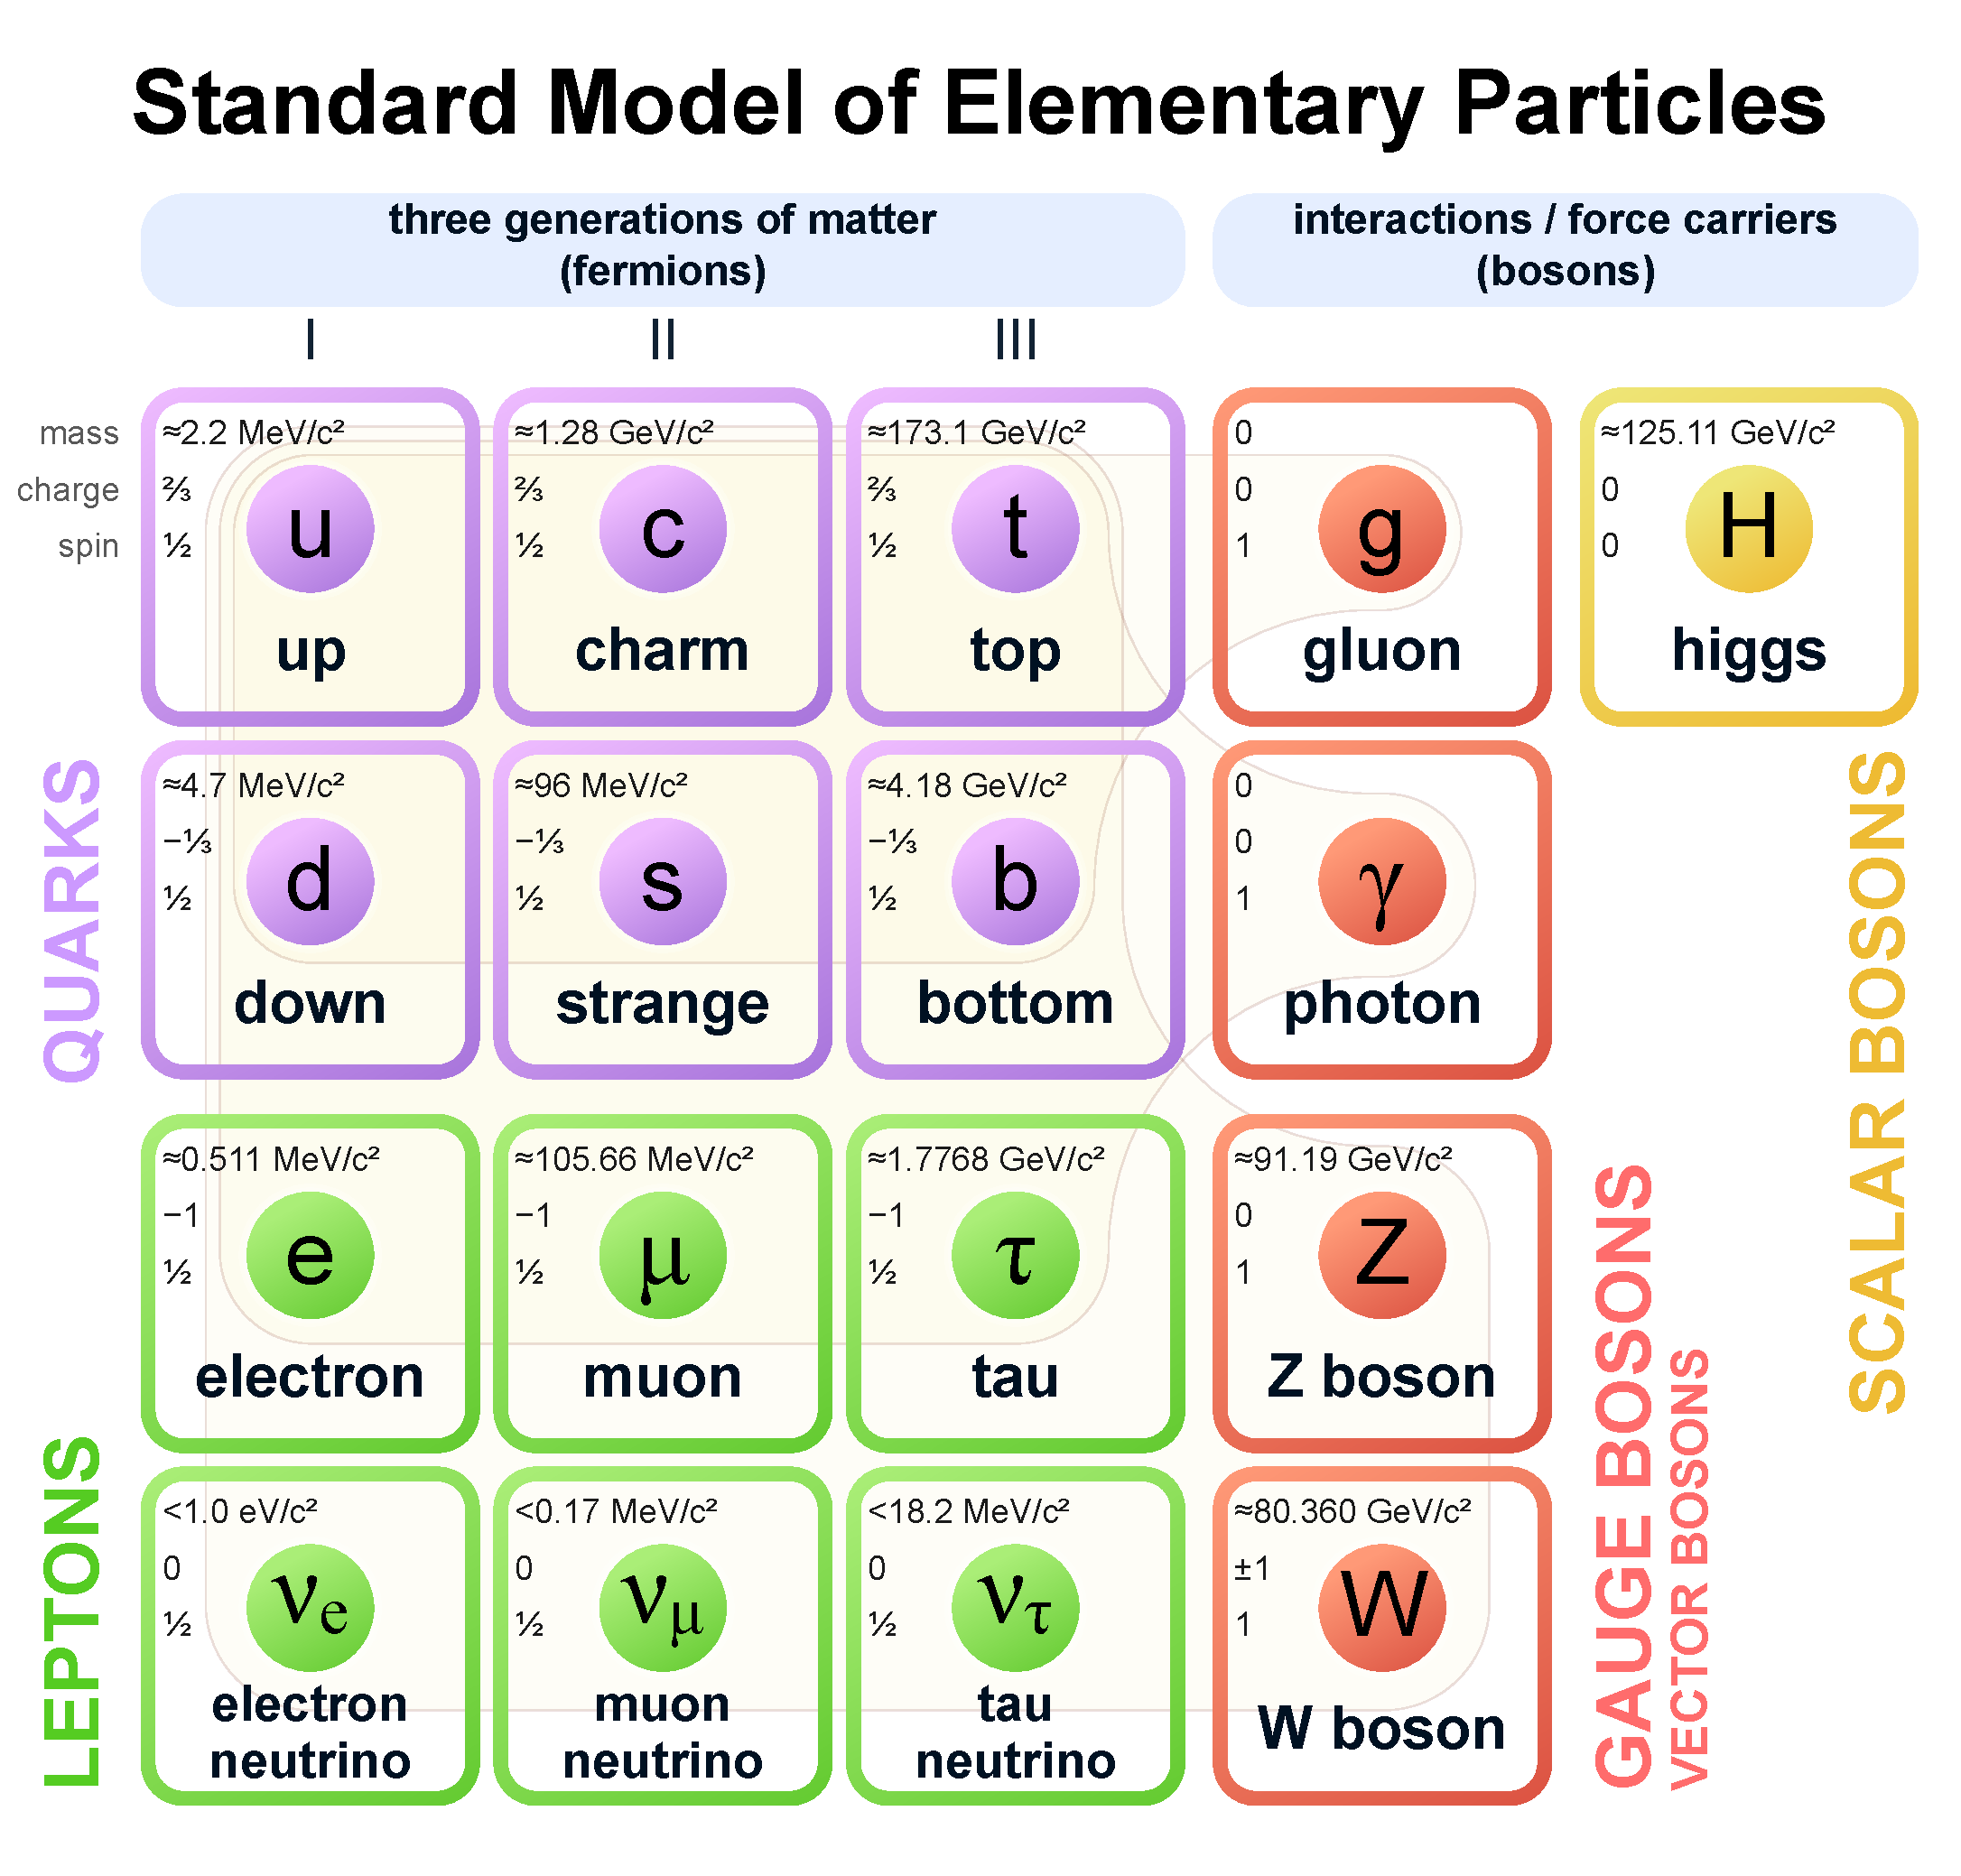
\includegraphics[width =0.8\textwidth]{figures/pdf/Standard_Model_of_Elementary_Particles.pdf}
\caption{Elementary particles of the Standard Model.}
\label{fig:sm}
\end{figure}


\subsubsection{Bosons}\label{bosons}
A boson is a particle with zero or integer spin, which follows Bose-Einstein statistics.
There are twelve fundamental bosons, that are the mediators of interactions as the $\gamma$, $Z$, $W^{\pm}$ for the electroweak interaction and as the eight gluons for the strong interaction.
The Higgs is a complex scalar weak isospin doublet that is responsible for the mechanism through which fermions and
bosons acquire mass and also explains the origin of $U (1)_{EM}$ through the spontaneous
symmetry breaking of the $SU (2)_L \times SU (1)_Y$ in the electroweak sector. Also mesons, that are composed of a quark and antiquark pair, are bosons. Bosons can be either massive, as $Z$, Higgs and $W^{\pm}$, or massless, as the photon and gluons.

\subsubsection{Fermions}
A fermion is a particle characterized by a non-integer spin, i.e. $1/2$, $3/2$ and follows the Fermi-Dirac statistics. The Pauli exclusion principle must be respected. Fermions are divided in two categories, leptons and quarks, depending on the forces through which they interact.  The arrangement of fermions into three generations is dictated by various properties, including mass among other properties, with more massive particles assigned to higher generations, as depicted in Fig.\ref{fig:sm}. Particles of the second and third generations exhibit instability and decay into first-generation particles. Leptons do not interact through strong interaction because they are not color charged, so they interact only via weak and electromagnetic interaction. They are categorized into two groups based on the electric charge: $e$, $\mu$, $\tau$ are the charged leptons and $\nu_e$, $\nu_{\mu}$, $\nu_{\tau}$ are the neutral ones. These particles form doublets of flavour. Neutrinos, due to their neutral nature, interact only weakly so their detection is extremely challenging. The six quarks participate in all known interactions. The known quarks are, in ascending order of mass and generation: up ($u$) and down ($d$), strange ($s$) and charm ($c$), bottom ($b$) and top ($t$) and their antiparticles. They primarily interact with each other through the strong force by gluons exchange. Free quarks have never been observed due to confinement, since they carry color charge. Confinement of quarks is a fundamental aspect of the theory of quantum chromodynamics (QCD) which describes the strong nuclear force. Quarks combine to form color-neutral particles known as hadrons, classified into baryons and mesons. Baryons consist of an odd number of quarks, while mesons, as mentioned in Subsection \ref{bosons}, are composed of a quark and an antiquark. Since quarks have weak electric charge and isospin, they can interact with each other and other fermions through weak and electromagnetic interactions.

\subsection{History of flavor}
The concept of flavor, namely the presence of three duplicates for every family of elementary fermions, is a fundamental aspect in particle physics. This principle is implemented within the Standard Model by introducing three copies of the gauge representations of fermion fields. This view began to take shape in the late 1940s. The origin can be traced back to the experiment conducted by Conversi, Pancini and Piccioni in 1947. These experiment revealed that negative muons, called at that time $mesotrons$, did not undergo nuclear capture as expected. They decayed in electrons, similarly to positive muons, therefore they could not be Yukawa particles. In the same year, Powell and his group identified a two-step decay process ($\pi \rightarrow \mu \rightarrow e$), distinguishing the pion from the muon. Bruno Pontecorvo suggested that the muon could be a sort of $isomer$ of the electron, leading to the idea of a second generation of elementary fermions. Rochester and Butler discovered unusual events in cosmic rays pictures, later identified as $V-particles$ (later discovered that they originated from neutral kaons). This was the first hint of the existence of a second generation of quarks. In 1950 the search for decay $\mu \rightarrow e \gamma$ began. This decay was not found, leading to the principle of conservation of leptons. On the hadron side, the second generation of quarks was established in the mid-70s, involving the GIM mechanism and the discovery of the charm quark. Meanwhile, on the leptonic side, the upper limit on the branching ratio of $\mu^+ \rightarrow  e^+ \gamma$ was set in 1955. The discovery of parity violation in the late 1950s suggested the weak interaction is mediated by bosons. \textit{Feinberg started thinking that $\mu^+ \rightarrow  e^+ \gamma$ could occur at a level of $10^{-4}$ if the bosons existed, through a loop with neutrino and a boson}. This lead to the two-neutrino hypothesis, suggesting that the neutrino coupled to the muon differs from that coupled to the electron, thereby prohibiting $\mu^+ \rightarrow  e^+ \gamma$. The existence of two neutrinos was verified at Brookhaven National Laboratory, with the scattering of two neutrinos coming from $\pi$, that produced only muons. After the observation of CP violation in neutral kaon decay, a third generation of quarks was hypothesized. After the discoveries of the $\tau$ (1976), the $b$ quark (1977), $t$ quark (1995) and $\nu_{\tau}$ (2000), a complete picture was achieved and the concept of flavor was consolidated in the Standard Model.


\subsection{Overview of CLFV}
There are three different lepton flavors: the electron-lepton number $L_e$, the muon-lepton number $L_{\mu}$ and the tau-lepton number $L_{\tau}$. In Table \ref{tab:leptons}, the quantum numbers assigned to each lepton are displayed.
 \begin{center}  
\begin{table}[!h]
\centering
\renewcommand{\arraystretch}{1.5}
\begin{tabular}{c c c c}
\hline
Lepton & $L_e$ & $L_{\mu}$ & $L_{\tau}$\\
\hline
$e^-/e^+$ & $+1 \ /-1$ & 0 & 0 \\
$\nu_{e}/\bar{\nu}_{e}$ & $+1 \ /-1$ & 0 & 0 \\
$\mu^-/\mu^+$ & 0 & $+1 \ /-1$ & 0 \\
$\nu_{\mu}/\bar{\nu}_{\mu}$ & 0 & $+1 \ /-1$ & 0 \\
$\tau^-/\tau^+$ & 0 & 0 & $+1 \ /-1$\\
$\nu_{\tau}/\bar{\nu}_{\tau}$ & 0 & 0 & $+1 \ /-1$ \\
\hline
\end{tabular}
\caption{Lepton numbers assigned to neutrinos and charged leptons.}
\end{table}\label{tab:leptons}
\end{center}
In the Standard Model (SM) defined with massless left-handed neutrinos, Lepton Flavor (LF) is a conserved quantity, Ref. \cite{universe8060299}. Experimental observations have demonstrated that, as they travel, neutrinos exhibit flavor oscillations, which implies that they must have non-zero masses and mixing angles. This phenomenon represents also a violation of the conservation of the lepton flavor. The Standard Model, while successful in many aspects, fails to explain phenomena like neutrino masses and the consequent flavor oscillations. Since neutrinos get their masses through renormalizable Yukawa interactions
with the Higgs, the predicted CLFV transitions are suppressed by sums over $(\Delta m^2_{i j}/M^2 _W)^2$, as calculated in Ref. \cite{MARCIANO1977303} and as shown in Section \ref{massiveneutrinos}, where $\Delta m^2_{ij}$ is mass-squared difference between the neutrino mass eigenstates $i$, $j$ and $M_W$ is the $W$ boson mass. The neutrino mass difference is very small ($\Delta m^2 _{i j} \leq 10^{-3}$ eV$^2$) with respect to the $W$ boson mass so the expected branching ratios reach unmeasurable values, below $10^{-50}$. Experimental studies of the lepton flavor violating process could open a window to new physics. Moreover, lepton flavor constitutes an accidental symmetry within the SM, not related to the gauge structure of the theory but coming
from its particle content, especially from the absence of RH neutrinos. Minor deviations from the Standard Model can easily give rise to extra occurrences of lepton flavor violation, leading to notable rates of CLFV.
There are various extensions of the Standard Model that could potentially be examined in the upcoming experimental searches for CLFV.
In Section \ref{leptonsector}, I will talk about lepton sector and how the lepton numbers are conserved. In Section \ref{massiveneutrinos}, a brief introduction of CLFV with massive neutrinos will be given.
In Section \ref{2higgs} and in Section \ref{susy}, I present a short discussion on Two Higgs Doublet Model and the CLFV in Super-symmetry respectively.
\subsection{Lepton sector in Standard Model}\label{leptonsector}
In the SM, only one Higgs field $\Phi$ exists. The fermions masses and the mixing term arise from the couplings of fermions with Higgs field. In the following, I will call the left-handed $i$-th quarks doublets and leptons doublets as $Q_{L,i}=(u_{L,i} \ d_{L,i})^T$ and $L_{L,i}=(\nu_{L,i} \ e_{L,i})^T$: $u_i$ will be the up-type quark, $d_i$ the down-type quark, $\nu_i$ the neutrino and $e_i$ the charged lepton. These are $SU(2)$ doublets, while $u_{R,j}$, $d_{R,j}$ and $e_{R,j}$ will be the right-handed up-type, down-type quarks and the right charged lepton of the $j$-generation respectively. There is no right-handed neutrino. The Yukawa coupling of fermions with the Higgs field $\mathscr{L}_Y$ is the sum of two terms: $\mathscr{L}_e$ that describes the leptonic component (Eq.\ref{leptoniccomponent}) and $\mathscr{L}_q$ that describes the quark one (Eq.\ref{quarkcomponent}).
\begin{equation}\label{leptoniccomponent}
    -\mathscr{L}_e=\left(Y_e\right)_{i j} \bar{L}_{L i} e_{R j} \Phi+ \text{ h.c. }
\end{equation}
\begin{equation}\label{quarkcomponent}
        -\mathscr{L}_q=\left(Y_u\right)_{i j} \bar{Q}_{L i} u_{R j} \widetilde{\Phi}+\left(Y_d\right)_{i j} \bar{Q}_{L i} d_{R j} \Phi+\text { h.c. }
\end{equation}

where the term $Y_f \ (f  =  u,d,e)$ describe the 3$\times$3 Yukawa complex matrices. $\widetilde{\Phi} \equiv i \tau_2 \Phi^*$ is the conjugate Higgs field. The mass terms of fermions, characterized by the $m_f \bar{f}_L f_R$ form, originate from the breaking of the $SU(2)_L \times U(1)$ symmetry caused by the vacuum expectation value of the Higgs field, as in Eq.\ref{higgs}.
\begin{equation}\label{higgs}
\langle\Phi\rangle=\frac{1}{\sqrt{2}}\left(\begin{array}{l}
0 \\
v
\end{array}\right) \qquad v \simeq 246 \mathrm{GeV}
\end{equation}
The fermion mass is given by:
\begin{equation}
\left(m_f\right)_{i j}=\frac{v}{\sqrt{2}}\left(Y_f\right)_{i j} \qquad f=u, d, e
\end{equation}
Since a right-handed neutrino does not appear in the Lagrangian, neutrinos have no mass, as it is formulated in the SM. The Yukawa matrices can be diagonalized through unitary rotations of the fields, as it follows:
\begin{equation}
Y_f=V_f \hat{Y}_f U_f^{\dagger} \qquad f=u, d, e
\end{equation}
where $ \hat{Y}_f $ is the diagonal Yukawa matrix. It is possible to label fermions in the rotated basis as $f^{\prime}$, so $f_L=V_f f^{\prime}_L$ and $f_R=V_f f^{\prime}_R $. Since $V_f$ and $U_f$ are unitary, the rotation will not affect the neutral interactions term and the kinetic terms, as we can see in $\bar{f}_L \gamma^\mu f_L=\bar{f}_L \gamma^\mu\left(V_f^{\dagger} V_f\right) f_L=\bar{f}_L^{\prime} \gamma^\mu f_L^{\prime}$. The coupling between fermion and Higgs boson will be:
\begin{equation}
-\mathscr{L}_{h \bar{f} f}=\frac{(\hat{m}_f)_{i j}}{v} \bar{f}_{L i}^{\prime}f^{\prime}_{R j} h+\text{h.c.} \qquad f=u, d, e
\end{equation}
where $\hat{m}_f$ denotes the diagonalized mass matrix: it is clear that there are no flavor-violating terms.
In quark sector flavor-violation arises from the rotations in Eq.\ref{quarkviolation} in the charged-current interactions with the $W$ bosons:
\begin{equation}\label{quarkviolation}
\begin{array}{c}
      { \displaystyle 
\mathscr{L}_{C C}  =\frac{g}{\sqrt{2}}\left(\bar{u}_L \gamma^\mu d_L+\bar{\nu}_L \gamma^\mu e_L\right) W_\mu^{+}+\text {h.c.} }\\
 {\displaystyle=\frac{g}{\sqrt{2}}\left(\bar{u}^{\prime}_L \gamma^\mu\left(V_u^{\dagger} V_d\right) d_L^{\prime}+\bar{\nu}^{\prime}_L \gamma^\mu\left(V_\nu^{\dagger} V_e\right) e_L^{\prime}\right) W_\mu^{+}+\text {h.c.}}
\end{array}
\end{equation}

The violation comes from the fact that $V_u \neq V_d$. The mixing is controlled by the Cabibbo-Kobayashi-Maskawa matrix $V_{CKM}\equiv V^{\dagger}_u V_d $, Ref. \cite{PhysRevLett.10.531}. Meanwhile, as the lepton sector contains massless neutrinos, $V_{\nu}$ can be arbitrarily chosen as $V_{\nu}=V_e$. From the preceding discussions, it becomes evident that in the SM with massless neutrinos, there is no occurrence of LFV in any form. The Lagrangian $\mathscr{L}_Y$ is invariant under three indipendent global $U(1)$ rotations, resulting in the conservation of three lepton family numbers: $L_e$, $L_\mu$ and $L_\tau$. Furthermore, if the Yukawa coupling Lagrangian includes supplementary terms involving the lepton fields, flavor violation can occur in the lepton sector. Examples of such additions could be a neutrino mass term or a second Higgs doublet.

\subsection{CLFV in the Standard Model with massive neutrinos}\label{massiveneutrinos}
The first evidence against the hypotesis of massless neutrinos emerged with the solar neutrino problem. In the 1960s, the solar neutrino detection experiment at Homestake revealed that the observed number of solar neutrinos, generated by fusion in the Sun, was significantly lower than the anticipated value based on the standard solar model, given that the detector was only sensitive to $\nu_e$, Ref. \cite{PhysRevLett.20.1205}. Consistent results were replicated in subsequent experiments employing radiochemical and Cherenkov detectors, discovering neutrino oscillations. These oscillation firmly established non-zero neutrino masses. The lepton flavor-violating neutrino oscillations showed that the global $U(1)$ symmetries associated with the lepton family numbers are not fundamental symmetries. A correction to standard model is needed to include neutrino mass terms. This is possible adding a right-handed neutrino singlet $\nu_R$ or some non-renormalizable operators.
\\
In the first case, an additional term $\Delta \mathscr{L}_D$ to the Yukawa coupling should be introduced:
\begin{equation}
-\Delta \mathscr{L}_D=\left(Y_\nu\right)_{i j} \bar{L}_{L i} \nu_{Rj} \widetilde{\Phi}+\text { h.c. }
\end{equation}
Similarly to other fermions, a Dirac mass term $m_{\nu} \bar{\nu}_L \nu_R$ is generated through simmetry breaking:
\begin{equation}
\left(m_\nu^D\right)_{i j}=\frac{v}{\sqrt{2}}\left(Y_\nu\right)_{i j}
\end{equation}
In this case, the small neutrino masses can be explained only if a very small term $Y_\nu$ is considered ($\leq 10^{-12}$), Ref. \cite{clfv_signorelli}. This brings us considering the second hypotesis: adding non-renormalizable operators can introduce Majorana masses for left-handed neutrinos alone. The corresponding $\Delta \mathscr{L}_M$ can be written as:
\begin{equation}
-\Delta \mathscr{L}_M=\frac{1}{2}\left(m_\nu^M\right)_{i j} \overline{\nu_{L i}^C} \nu_{L j}+\text{ h.c.}
\end{equation}
where $\overline{\nu_{L }^C} $ is the charge-conjugated fields. This term violates lepton number and requires an operator of dimension 5, Ref. \cite{wein}, to be consistent with SM symmetries. A minimal Lagrangian is given by:
\begin{equation}
-\Delta \mathscr{L}_{M \text { eff}}=\frac{\mathcal{C}_{i j}}{\Lambda}\left(\overline{L_{L i}^C} \tau_2 \Phi\right)\left(\Phi^T \tau_2 L_{L j}\right)+\text { h.c.}
\end{equation}
where the $\Lambda$ term represents a mass scale characteristic of extra degrees of freedom and the $C_{ij}$ is an antisymmetric charge conjugation matrix. The corresponding Majorana mass term is:
\begin{equation}
\left(m_\nu^M\right)_{i j}=\frac{\mathcal{C}_{i j} v^2}{\Lambda}
\end{equation}
In this case, the small neutrino masses can be explained only if $\Lambda > > v$: this seems to appear more natural than the previous case. No matter how the extra neutrino mass factor is expressed precisely, a physical basis diagonalizing the mass matrix is determined, resulting in $V_{\nu} \neq V_e$ in Equation \ref{quarkviolation}. Lepton mixing is described by $U_{PMNS} \equiv V_{\nu}^{\dagger} V_e$, which is similar to the CKM matrix. The Pontecorvo-Maki-Nakagawa-Sakata (PMNS) matrix is the term that is typically used to refer to it. As it is in the basis diagonalizing charged lepton masses and it diagonalizes the neutrino mass matrix, $U_{PMNS}$ also explains the mixing between neutrino flavor eigenstates $\nu_{\alpha}$ and mass eigenstates $\nu_i$:
\begin{equation}
\nu_\alpha=\sum_{i=1,2,3}\left(U_{\mathrm{PMNS}}\right)_{l i} \ \nu_i \qquad l=e, \mu, \tau
\end{equation}
In addition to the neutral LFV observed in neutrino oscillations, the mixing outlined by $U_{PMNS}$ can in principle give rise to processes known as Charged Lepton Flavor Violations, i.e. LFV that involves charged leptons. The new Feynman diagrams are loops involving neutrinos and $W$ bosons, as $\mu \rightarrow e \gamma$ in Fig.\ref{fig:mutoegamma} and $\mu N \rightarrow e N$ in Fig.\ref{fig:mutoeN}. 



\begin{figure}[!h]
     \begin{subfigure}[b]{0.4\linewidth}
         \centering
         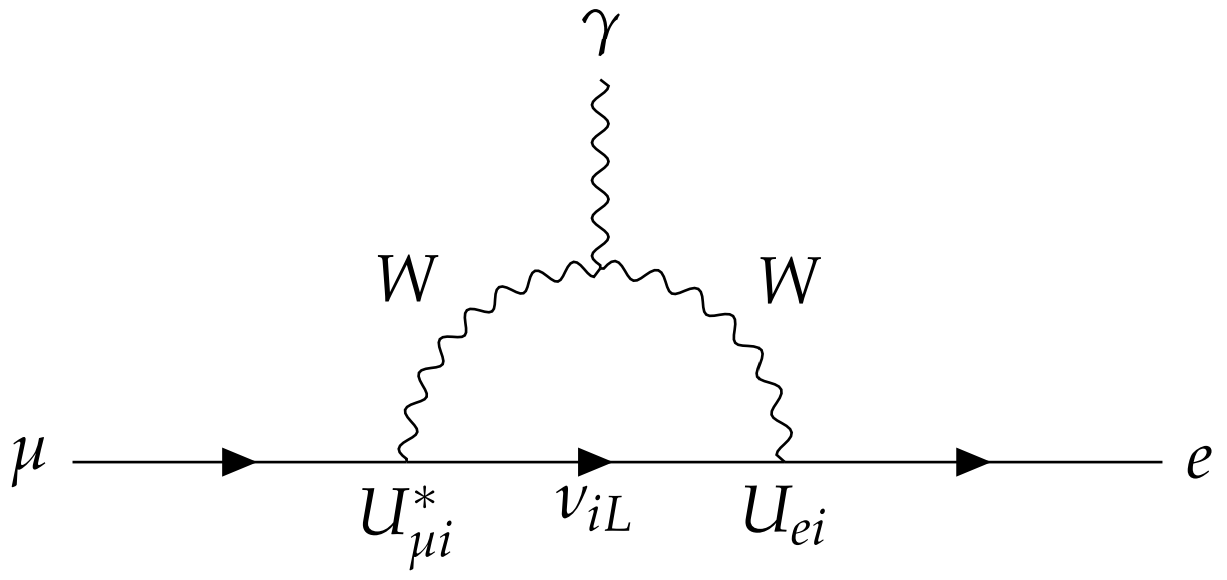
\includegraphics[scale = 0.2]{figures/png/Screenshot_20240217_171058.png}
         \subcaption{$\mu \rightarrow e \gamma$ process, Ref. \cite{universe8060299}.}
         \label{fig:mutoegamma}
     \end{subfigure}
     \begin{subfigure}[b]{0.7\linewidth}
         \centering
         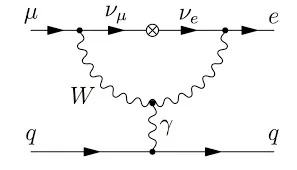
\includegraphics[scale = 0.5]{figures/jpg/1_erkKoywyuFzJmMv4PKpc9Q.jpg}
         \subcaption{$\mu N \rightarrow e N$ process.}
         \label{fig:mutoeN}
     \end{subfigure}
     \caption{Some of CLFV processes.}
        \label{fig:three graphs2}
\end{figure}
In the SM, each of these mechanisms is significantly inhibited. Using the example of $\mu \rightarrow  e \gamma $, the branching ratio of this process may be computed as follows:

\begin{equation}\label{br}
\begin{aligned}
B R(\mu \rightarrow e \gamma) & =\frac{3 \alpha}{32 \pi}\left|\sum_{i=2,3} U_{\mu i}^* U_{e i} \frac{\Delta m_{1 i}^2}{M_W^2}\right|^2 \\
& =\frac{3 \alpha}{32 \pi}\left(\frac{1}{4}\right) \sin ^2 2 \theta_{13} \sin ^2 \theta_{23}\left|\frac{\Delta m_{13}^2}{M_W^2}\right|^2
\end{aligned}
\end{equation}

where $\alpha$ is the fine structure constant, $U_{\mu i}$ and $U_{ei}$ are corresponding elements in the PMNS matrix, $\Delta m_{1i}^2$ is the neutrino squared mass differences, $M_W$ is the $W$ boson mass and $\theta_{13}$ and $\theta_{23}$ are rotating angles in PMNS matrix parametrization. The expression yields $B R(\mu \rightarrow e \gamma) \sim \mathcal{O}(10^{-54})$. The big discrepancy in mass between neutrinos and the $W$ boson results in an extraordinarily small value for $|\Delta m_{13}^2/M_W|$. Equivalent suppression mechanisms are evident in other CLFV processes. The rates predicted by the Standard Model are extremely small, making them impractical for detection in any experiment. On the other hand, numerous Beyond the Standard Model (BSM) theories incorporate mechanisms that substantially amplify CLFV rates, a topic to be addressed in the subsequent section. The small value of SM CLFV rates implies that the detection of any CLFV processes in experiments would unequivocally indicate the presence of physics beyond the SM.
\subsection{Beyond the Standard Model}
Numerous Beyond the Standard Model (BSM) theories propose mechanisms that could contribute to CLFV processes, potentially yielding detectable rates in experiments. Here, we highlight a selection of BSM theories known for their CLFV contributions. It is important to note that this list is not comprehensive; for further studies, additional reviews are available in Ref. \cite{clfv_signorelli} and Ref. \cite{universe8060299}.
\subsubsection{CLFV in Supersymmetry}\label{susy}
Supersymmetry (SUSY) is a theoretical framework that has oriented experiments in the CLFV reasearch for many years. On one hand, models with SUSY broken at energies close to electro-weak scale have given solution to the hierarchy problem, i.e. how to maintain the Higgs mass significantly smaller than the Planck scale ($\sim$10$^{19}$ GeV). On the other hand, the suppression of CLFV processes is due to the wide separation of the neutrinos and $W$ masses, which can be mitigated by introducing SUSY partners of neutrinos and $W$ bosons. This suggests that CLFV processes should have been observable earlier, unless SUSY breaking occurs at or near the electroweak scale ($\sim 10^2$ GeV), Ref. \cite{clfv_signorelli}. In this framework, each elementary particle has a superpartner,  with the same quantum numbers except for spin: a boson is the superpartner of a fermion and vice versa. A superpartner of a lepton is called $slepton$. If there is no common eigenstate base between lepton and $slepton$'s mass matrices then a physical $slepton$ will be a superposition of flavors. In this case a loop diagram can lead to CLFV, as shown in Fig.\ref{fig:susy}. Despite the similar topology to that of the SM contribution (Fig.\ref{fig:mutoegamma}), the typical SUSY mass is expected to be much higher than that of the neutrinos. Predictions for the branching ratio of this process vary among different SUSY models, contingent upon specific mechanisms and particle masses. These rates can undergo significant enhancement. For example, in an $SU(5)$ SUSY grand unified theory, the computed branching ratio could reach $\mathcal{O}(10^{-14})$ for a slepton mass on the order of $\mathcal{O}(10^{-14}$ GeV/c$^2)$, a value measurable for upcoming experiments.

\begin{figure}[!h]
\centering
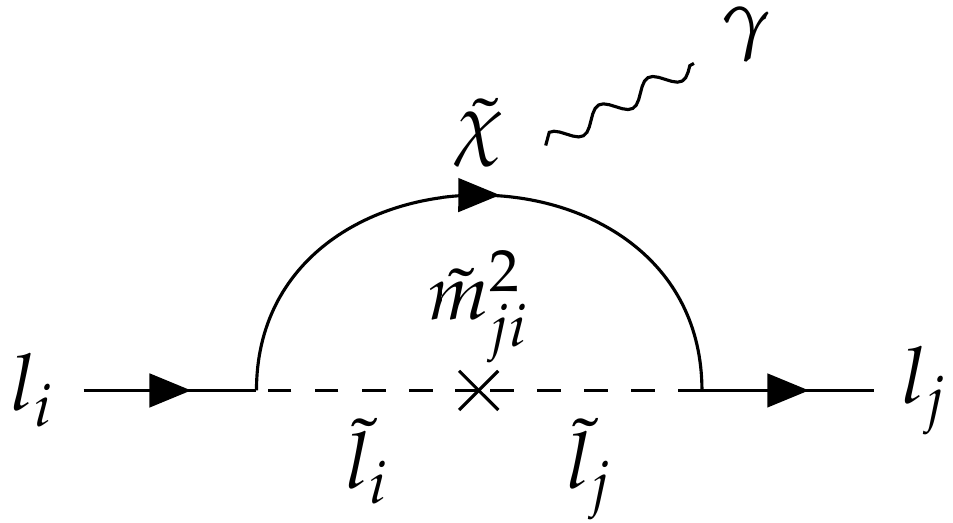
\includegraphics[width =0.4\textwidth]{figures/png/Screenshot_20240218_105920.png}
\caption{SUSY contribution to $l_i \rightarrow l_j\gamma$, through $sleptons$ mass mixing, Ref. \cite{universe8060299}.}
\label{fig:susy}
\end{figure}


\subsubsection{Two Higgs Doublet Model}\label{2higgs}
Although the Standard Model (SM) incorporates only one Higgs boson, there are no constraints against the presence of additional Higgs fields. One straightforward example of a comprehensive theory featuring multiple Higgs fields is the type III two Higgs doublet model (2HDM), where two Higgs bosons exist, each interacting with fermions and possessing a vacuum expectation value, Ref. \cite{Harnik_2013}. Generally, the Lagrangian incorporating extra Higgs fields post-electroweak symmetry breaking can be written as:
\begin{equation}
-\mathscr{L}=m_i \bar{f}_{L i} f_{R i}+\left(Y^\alpha\right)_{i j} \bar{f}_{L i} f_R{ }_j h^\alpha+\text { h.c. }+\ldots
\end{equation}
Non renormalizable terms of higher dimensions are omitted. $(Y^\alpha)_{i j}$ represents couplings to a single scalar field and the contributions from different Higgses are summed over. The non-zero-off-diagonal terms in $(Y^\alpha)_{i j}$ give rise to flavor violating Yukawa couplings. From accelerator and precision experiments, constraints on the off-diagonal coupling of the 125 GeV Higgs boson can be obtained.
\subsubsection{Leptoquark Models}
Leptoquarks (LQs) are theoretical particles initially proposed within the Pati-Salam model, Ref. \cite{PhysRevD.10.275}. Each LQ is linked to both baryon number ($B$) and lepton number ($L$). In various LQ models the quark and lepton sectors are unified. This unification allows for direct coupling between quarks and leptons via the exchange of LQs. Consequently, specific CLFV processes like $K_L^0 \rightarrow e \mu$ and $\mu N \rightarrow e N$ are mediated by LQs. Constraints on LQ models arise from both collider experiments and rare decay searches. Direct searches at ATLAS and CMS have excluded scalar LQs of the first and second generations with masses below $\sim$1 TeV. Indirect searches provide constraints on the mass-coupling plane, where regions with higher couplings and lower LQ masses correspond to higher branching ratios. Additionally, LQ models must satisfy constraints related to proton stability, as some models involve LQs that could mediate proton decay. To mitigate this, the corresponding LQs must either have extremely high masses or their related couplings must be exceedingly small, Ref. \cite{DORSNER20161}.
\subsubsection{Additional Neutral Gauge Boson}
Grand unified theories (GUTs) are constructed based on extended gauge groups in the pursuit of a more fundamental model. At lower energies, these extended gauge groups are believed to break down to the direct product of the Standard Model (SM) gauge group $SU(3) \times SU(2) \times U(1)$ along with an additional $U(1)$ factor. The neutral gauge boson associated with this $U(1)$ group can mix with the original SM neutral gauge boson, resulting in two mass eigenstates, namely $Z$ and $Z'$. Additionally, extended gauge theories require the introduction of additional fermion fields to cancel anomaly-free currents beyond those of $SU(5)$. These $new$ fermions can mix with the known SM fermions possessing the same electric and color charges, consequently affecting their couplings with gauge bosons. The appearance of off-diagonal terms in neutral current couplings to fermions can lead to flavor-changing couplings to $Z$ and $Z'$. Certain CLFV processes, such as $\mu \rightarrow eee$ and $\mu-e$ conversion, receive tree-level contributions through intermediate $Z$ and $Z'$ bosons. Further insights into the phenomenology of the $Z'$ boson can be found in, Ref. \cite{Leike_1999}. The search for the existence of $Z'$ bosons is conducted through channels like $Z' \rightarrow \bar{f}f$ at hadron colliders. Mass lower limits of $Z'$ from various specific models are listed in Ref. \cite{zyla}, primarily falling within the low TeV range. Particularly, mass lower limits reported in CLFV final states $e\mu$, $e\tau$ and $\mu\tau$ range between 3.5 TeV and 4.5 TeV. Upper limits of $Z \rightarrow l_1 l_2$ couplings to the normal $Z$ boson are also provided in Table \ref{tab:upperlimits}.
%Quello che segue è un esempio di codice. E' possibile modificare il linguaggio per il synyax highlight, aggiungere parole chiave... E' tutto disponibile nella guida del pacchetto \texttt{listings}.

%\lstinputlisting[language=C++]{listings/png/code1.cpp} 
\section{Experiments looking for CLFV}
CLFV has not been observed yet, despite ongoing efforts to detect such violations in different channels in both dedicated and general-purpose experiments. 
Some of these efforts are documented in Table \ref{tab:upperlimits}, which presents their respective experimental upper limits. 
In addition to searches at collider experiments, such as observing $Z$ and 
Higgs decays, rare decay experiments play a significant role as a complementary method in the search for CLFV. 
Collider experiments enable the exploration of various CLFV channels simultaneously, including those involving $\tau$s. 
However, complexities in data selection and reconstruction and limitations in statistics present challenges to improve the limits in this field.
Rare decay experiments, by focusing on specific processes or a set of similar processes, can achieve high statistics using an intense particle beam. 
By suppressing background signals, these experiments can significantly improve sensitivity. Furthermore, this approach 
enables the investigation of high mass scales, as will be explained in the next section. 
\begin{center}  
\begin{table}[!h]
\centering
\renewcommand{\arraystretch}{1.5}
\begin{tabular}{c c c c c c}
\hline
Reaction & Present limit & C.L. & Experiment &  Year & Ref.\\
\hline
$\mu^+\ \rightarrow \ e^+ \ \gamma$& $7.5 \times 10^{-13}$ & 90\% & MEG II & 2024 & \cite{megiicollaboration2024search}\\
$\mu^+ \ \rightarrow \ e^+ \ e^+ \ e^-$ & $1.0 \times 10^{-12}$ & 90\% & SINDRUM & 1988 & \cite{SINDRUM:1987nra} \\
$\mu^- \ \text{Ti}\ \rightarrow \ e^- \ \text{Ti}$ &  $6.1 \times 10^{-13}$ & 90\% & SINDRUM II & 1998 & \cite{titanium}\\
$\mu^- \ \text{Au}\ \rightarrow \ e^- \ \text{Au}$ & $7.0 \times 10^{-13}$ & 90\% & SINDRUM II & 2006 & \cite{SINDRUMII:2006dvw} \\
$\mu^+ \ e^- \ \rightarrow \ \mu^- \ e^+$ & $8.3 \times 10^{-11}$ & 90\% & SINDRUM & 1999 & \cite{Willmann:1998gd}\\
$\tau \ \rightarrow \ e \ \gamma$ & $3.3 \times 10^{-8}$ & 90\% & BaBar & 2010 & \cite{Aubert_2010}\\
$\tau \ \rightarrow \ \mu \ \gamma$ & $4.4 \times 10^{-8}$ & 90\% & BaBar & 2010 & \cite{Aubert_2010}\\
$\tau \ \rightarrow \ e \ e \  e$ & $2.7 \times 10^{-8}$ & 90\% & Belle & 2010 & \cite{Hayasaka_2010}\\
$\tau \ \rightarrow \ \mu \ \mu  \ \mu$ & $2.1 \times 10^{-8}$ & 90\% & Belle & 2010 & \cite{Hayasaka_2010} \\
\hline
$B^0 \ \rightarrow \ \mu \ e$ & $2.8 \times 10^{-9}$ & 90\% & LHCb & 2013 & \cite{PhysRevLett.111.141801}\\
$B^0 \ \rightarrow \ \tau \ e$ & $2.8 \times 10^{-5}$ & 90\% & BaBar & 2008 & \cite{PhysRevD.77.091104}\\
$B^0 \ \rightarrow \ \tau \ \mu$ & $2.2 \times 10^{-5}$ & 90\% & BaBar & 2008 & \cite{PhysRevD.77.091104}\\
$K_L^0 \ \rightarrow \ \mu \ e$ & $4.7 \times 10^{-12}$& 90\% & BNL E871 & 1998 & \cite{BNL:1998apv}\\
$K^+\ \rightarrow \ \pi^+ \ \mu^+ \ e^-$ & $2.1 \times 10^{-10} $ & 90\% & BNL E865 & 2005 & \cite{PhysRevD.72.012005}\\
$K_L^0 \ \rightarrow \ \pi^0 \ \mu^+ \ e^-$ & $ 4.4 \times 10^{-10}$ & 90\% & KTeV & 2008 & \cite{KTeV:2007cvy}\\
$\pi^0 \ \rightarrow \ \mu \ e$ & $8.6 \times 10^{-9}$ & 90\% & KTeV & 2008 & \cite{KTeV:2007cvy}\\
$\Upsilon (1s) \ \rightarrow \ \mu \ \tau $ & $6.0 \times 10^{-6}$ & 95\% & CLEO & 2008 & \cite{Love_2008}\\
\hline
$Z^0 \ \rightarrow \ \mu \ e$ & $1.7 \times 10^{-6}$ & 95\% &  LHC ATLAS & 2014 & \cite{Aad_2014} \\
$Z^0 \ \rightarrow \ \tau \ e$ & $1.7 \times 10^{-6}$ & 95\% &  LEP OPAL & 1995 & \cite{akers}\\
$Z^0 \ \rightarrow \ \tau \ \mu$ & $9.8 \times 10^{-6}$ & 95\% &  LEP DELPHI & 1997 & \cite{abreu}\\
$h \ \rightarrow \ e \ \mu$ & $3.5 \times 10^{-3}$ & 95\% & LHC CMS & 2016 & \cite{PhysRevD.104.032013}\\
$h \ \rightarrow \ \tau  \ \mu$ & $2.5 \times 10^{-3}$ & 95\% & LHC CMS & 2017 & \cite{cms17}\\
$h \ \rightarrow \ e \ \tau$ & $6.1 \times 10^{-3}$ & 95\% & LHC CMS & 2017 & \cite{cms17}\\
\hline
\end{tabular}
\caption{Experimental upper limits for a variety of CLFV processes of leptons, mesons and heavy bosons, Ref. \cite{clfv_signorelli}.}
\end{table}\label{tab:upperlimits}
\end{center}


\subsection{$\mu$ Channels}
Currently, the most promising channel is the one that includes muon processes. When a proton beam interacts with a target, 
pions and kaons are produced, that subsequently decay in muons. Muon lifetime is long enough to form a muon beam and we are able to reach 
intensities of 10$^8 \div 10^{11} \  \mu$/s. There are three primary CLFV channels involving muons, with distinct sensitivities to effective lagrangian 
terms: $\mu^+ \rightarrow e^+ \gamma$, $\mu^- N \rightarrow e^- N$ and $\mu^+ \rightarrow e^+ e^+ e^-$. The following paragraphs 
will discuss the experimental challenges and future perspectives for each of these channels. As seen in Table \ref{tab:upperlimits}, 
these channels have the lowest branching ratio limits. Muons have small mass, that results in a limited number of decay modes. Figure \ref{fig:muchannel} 
shows how the branching ratio limitations of muon uncommon decays have rapidly improved over the last several decades. The next-generation 
experiments aim to improve by many orders of magnitude. Muon rare decay studies can also provide theory differentiation power 
combining results of the three channels. All CLFV extensions to SM can be described by the following Lagrangian, Ref. \cite{doi:10.1146/annurev-nucl-100809-131949}:
\begin{equation}\label{LCF}
\begin{aligned}
\mathscr{L}_{C L F V}= & \frac{m_\mu}{(1+\kappa) \Lambda^2} \bar{\mu}_R \sigma_{\mu \nu} e_L F^{\mu \nu}+\text{h.c.}+ \\
&\frac{\kappa}{(1+\kappa) \Lambda^2} \bar{\mu}_L \gamma_\mu e_L\left(\sum_{q=u, d} \bar{q}_L \gamma^\mu \bar{q}_L\right)+\text{h.c.}
\end{aligned}
\end{equation}
$m_\mu$ is the muon mass and  $F^{\mu \nu}$ is the electromagnetic field tensor. This toy Lagrangian includes two parameters.
$\Gamma$ is the effective energy scale of the new physics and $\kappa$ is the relative strengths of the two operators. The first term in the Lagrangian 
is a magnetic-moment-type operator and describes all three processes mentioned above, it is generated by any loop with some new particle that can be either virtual and real.
The second one corresponds to a four-fermion operator, which mediates $\mu N \rightarrow eN$ at tree level and the other two processes at one-loop level.
The Mu2e experiment can probe an effective mass scale up to $\mathcal{O}$(10$^4$ TeV) with its designed sensitivity assuming $\kappa$ $\gg$ 1.
On the other hand, $\mu \rightarrow e\gamma$ experiments are more sensitive when $\kappa$ $\ll$ 1; the dominant magnetic
moment type term determines the other two processes have lower rates in such a case. In order to learn more about the new
physics, one needs to combine information involving the rates of a different CLFV processes, Ref. \cite{osti_1042577}.
The corresponding parameter space (the $\Gamma-\kappa$ plane) is shown in Figure \ref{fig:muchannelbr}, Ref. \cite{doi:10.1146/annurev-nucl-100809-131949}.
\begin{figure}[!h]
\centering
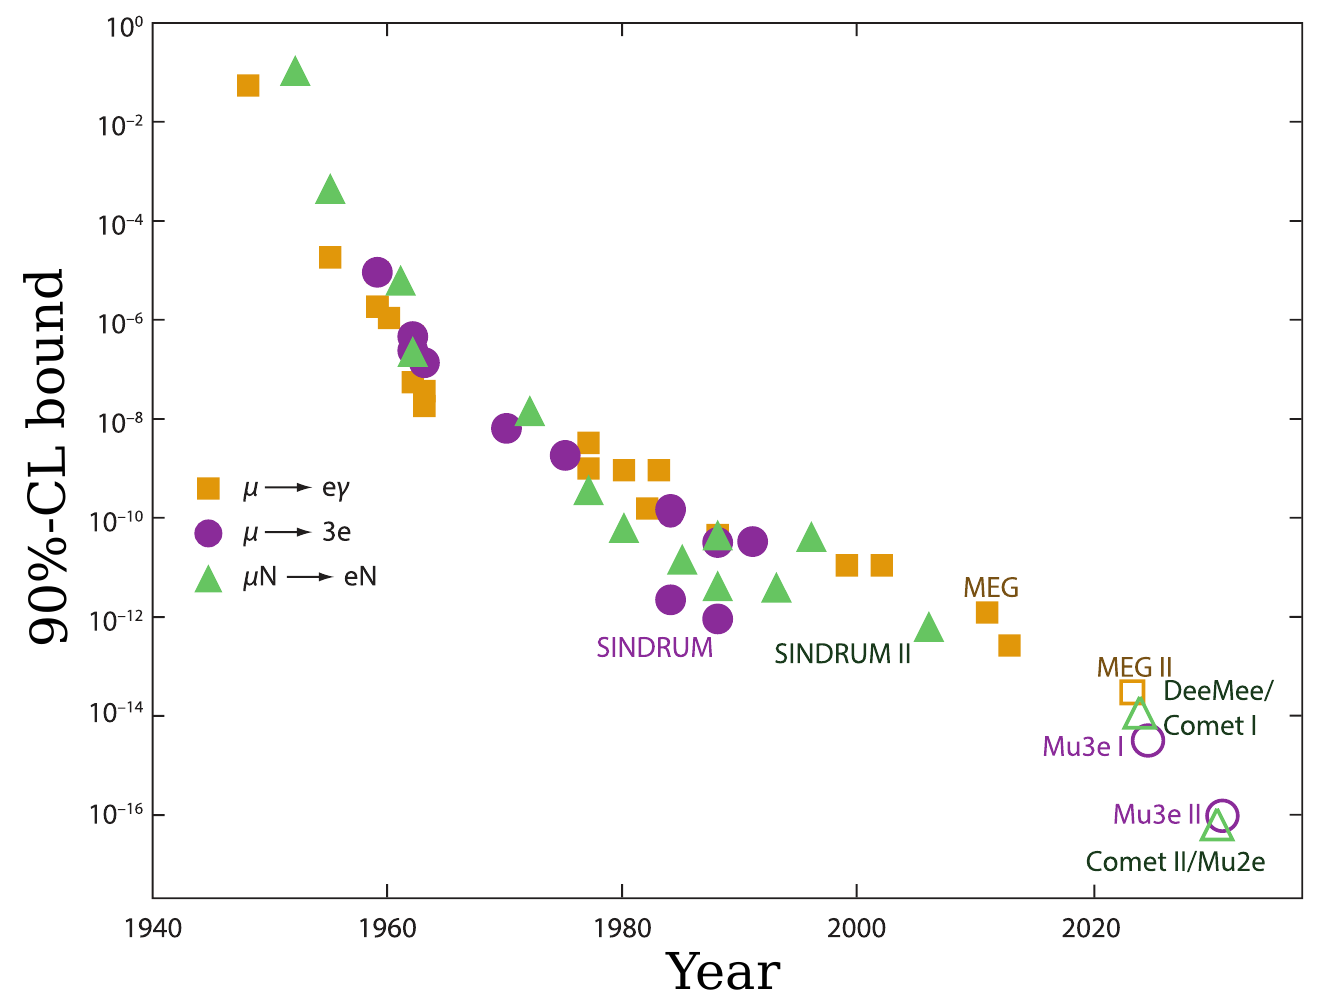
\includegraphics[width =0.7\textwidth]{figures/png/Screenshot_20240307_161549.png}
\caption{History and outlook of branching ratio limits in muon rare decay modes, Ref. \cite{MARCIANO1977303}.}
\label{fig:muchannel}
\end{figure}
\begin{figure}[!h]
\centering
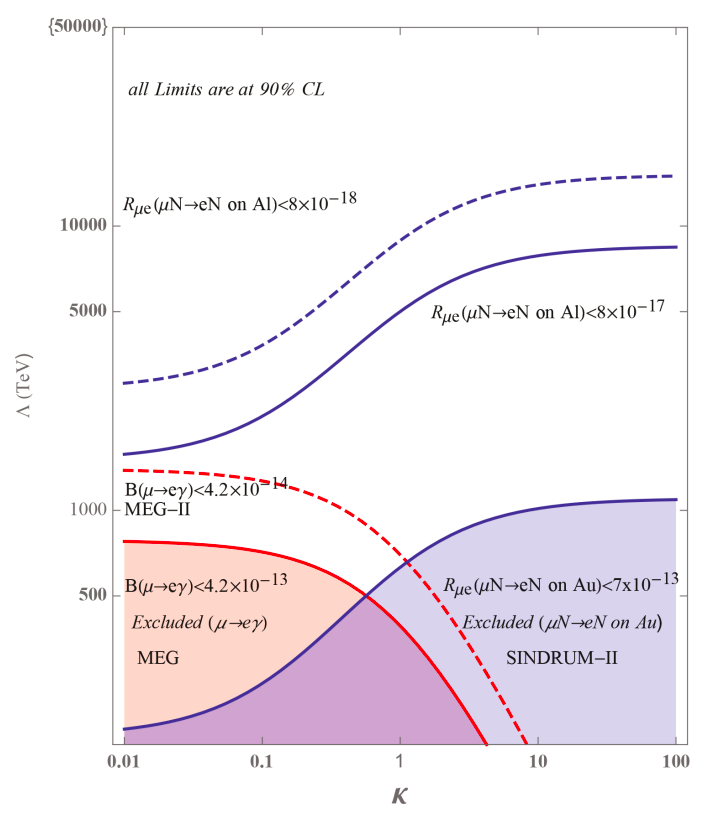
\includegraphics[width =0.7\textwidth]{figures/png/Screenshot_20240313_120457.png}
\caption{Sensitivity of $\mu \rightarrow e\gamma$ and $\mu N \rightarrow eN$ experiments to the new physics
scale $\Gamma$ as a function of $\kappa$ as defined in Equation \ref{LCF}, Ref. \cite{CGroup:2022tli}. The blue region is the New
Physics phase space excluded by SINDRUM-II, Ref. \cite{SINDRUMII:2006dvw}. The red region represents the
limit set by MEG, Ref. \cite{megi}, while the dashed red line represents the region that is
excluded by MEG-II, Ref. \cite{megiicollaboration2024search}. The solid (dashed) blu line is the
expected limit that would be set by Mu2e, Ref. \cite{universe9010054}.}
\label{fig:muchannelbr}
\end{figure}
\subsubsection{$\mu^+ \rightarrow e^+ \gamma$}
A clear signal of CLFV, in $\mu^+ \rightarrow e^+ \gamma$ channel, is given by back-to-back electron and photon, each one with energy of 52.8 MeV, 
both produced simultaneously. Positive muons are preferred since the negative ones may undergo the nuclear capture. 
Muons are stopped and decay at rest. There are two most significant sources of background: Radiative Muon Decay (RMD) $\mu^+ \rightarrow e^+ \nu_e \bar{\nu}_\mu \gamma$ 
and the accidental coincidence of $\mu^+ \rightarrow e^+ \nu_e \bar{\nu}_\mu$ with a random $\gamma$ 
generated by annihilation or bremsstrahlung. The first one is an in-time process, where neutrinos carry off a small part of the energy 
and it is only the 10\% of the total background. The accidental background is dominant. Since both backgrounds scale with the muon stop rate $\Gamma_\mu$, a continuous beam is preferred. 
Moreover, since an higher number of stopped muons correspond to a lower statistical error, but at the same time to a lower signal to background ratio, an optimal $\Gamma_\mu$ exists.
The stopping target thickness must optimized: a thin target is needed to minimise Multiple Coulomb Scattering, which affects the angular resolution of the outgoing electron, but 
it must be thick enough to block a significant portion of incoming muons. 
\paragraph{The MEG Experiment}
The MEG experiment, Ref. \cite{megi}, has been designed around two concepts: exploiting a liquid
xenon detector (LXe) for positron and photon tracking and an anti-bottle magnetic field, Ref. \cite{clfv_signorelli}. 
In Figure \ref{fig:meg}, the apparatus is shown. A polyethylene target is used to stop muons in the center of the magnet. 
The measured quantities are the electron and photon energies ($E_e$ and $E_\gamma$) and the
relative positions (angles $\theta_{e\gamma}$, $\phi_{e\gamma}$ and time $t_{e \gamma}$).
A combination of drift chambers (DCH) and plastic scintillator timing counters (TC) measures the positron momentum.
The photon energy and direction are measured in a volume of LXe with more than 800 photo-multipliers tubes. 
An energy resolution of less than 1\% for each particles is required to distinguish background from the signal. 
In MEG, the magnetic field decreases uniformly from centre to periphery, pushing particles away from the centre. 
The exact shape of the field has been chosen to have a track radius proportional to the absolute momentum.
This allows low energy positrons to be discarded by simply placing the detector far enough away from the magnet axis. 
This feature is unique to the MEG magnetic system and justifies its name as \textit{COnstant Bending RAdius} (COBRA) magnets.
The DCH spectrometer is composed by 16 trapezoidal drift chambers oriented radially and filled with He-C$_2$H$_6$. 
The timing from the DCH and TC is used to assess the radial coordinate, whereas the $z$ location is determined by measuring the induced
charged on the zig-zag shaped pads on the side of the drift chambers. The momentum resolution for $e^+$ is $\sim$ 330 keV.
A liquid xenon scintillating detector was used for photon reconstruction to reduce passive material and improve temporal resolution. 
This option provides more light yield than NaI crystals and has a substantially shorter decay period, with photon interaction times measured at less than 100 ps.
MEG collected $7.5 \times 10^{14}$ stopped muons in 2008-2013, setting a limit of $BR(\mu^+ \rightarrow e^+ \gamma) < 4.2 \times 10^{-13}$ at 90\% C.L., Ref. \cite{megi}.
\begin{figure}[!h]
\centering
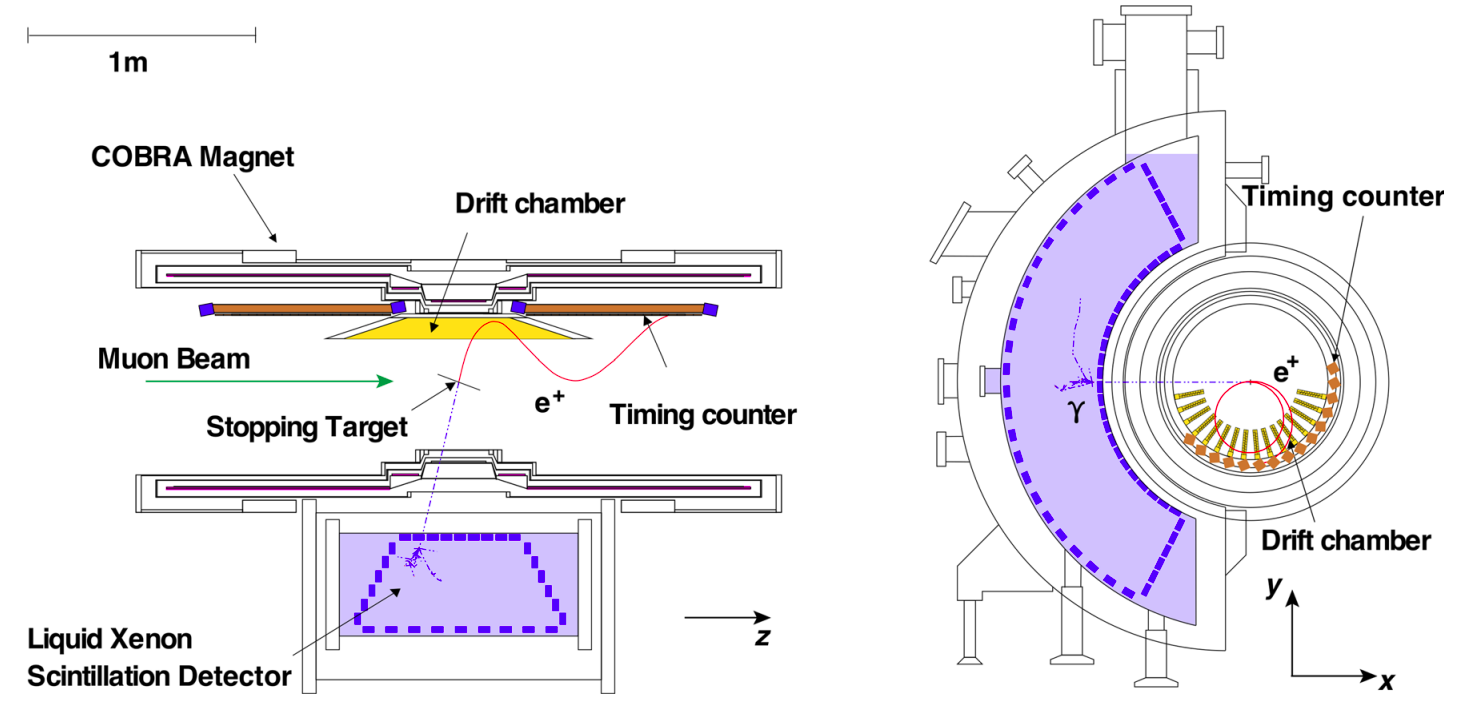
\includegraphics[width =0.8\textwidth]{figures/png/Screenshot_20240321_115127.png}
\caption{Schematic view of the MEG detector, Ref. \cite{megi}.}
\label{fig:meg}
\end{figure}
\paragraph{The MEG II experiment}
The MEG II detector is the upgrade to the MEG one, Ref. \cite{megiicollaboration2024operation}.
MEG II was proposed to reduce the contamination due to the accidental background that could not be further reduced in MEG.
In Figure \ref{fig:meg2}, the apparatus is shown. The muon flux was increased up to $7 \times 10^7 \ \mu^+$/s and a thinner but more inclined 
stopping target was installed to reduce the multiple scattering and bremsstrahlung 
while keeping the same stopping power (205 $\rightarrow$ 140 $\mu$m).
The old drift chamber was replaced with a new cylindrical drift chamber (CDCH) designed
to have higher granularity and transparency and made of 9 layers of drift cells to
improve positron track reconstruction. CDCH is shown in Figure \ref{fig:meg2}.
A more segmented system (pixellated-TC) was adopted instead of plastic scintillator timing counters (TC).
A Radiative Decay Counter was introduced, that is a target of scintillator and LYSO calorimeter positioned transversely to detect positron from RMD emitted at low angle.
When combined with the final result of MEG, MEG II collaboration obtained the most stringent limit up to date, $BR(\mu^+ \rightarrow e^+ \gamma)<3.1\times 10^{-13}$ 90\% C.L., Ref. \cite{megiicollaboration2024search}.
The MEG II collaboration took data in 2022 and 2023, collecting much more statistics compared to 2021. By 2026, more than twenty-fold increase in statistics is foreseen, with the goal of reaching a
$BR(\mu^+ \rightarrow e^+ \gamma)\lesssim 6\times 10^{-14}$ 90\% C.L..
\begin{figure}[!h]
    \centering
    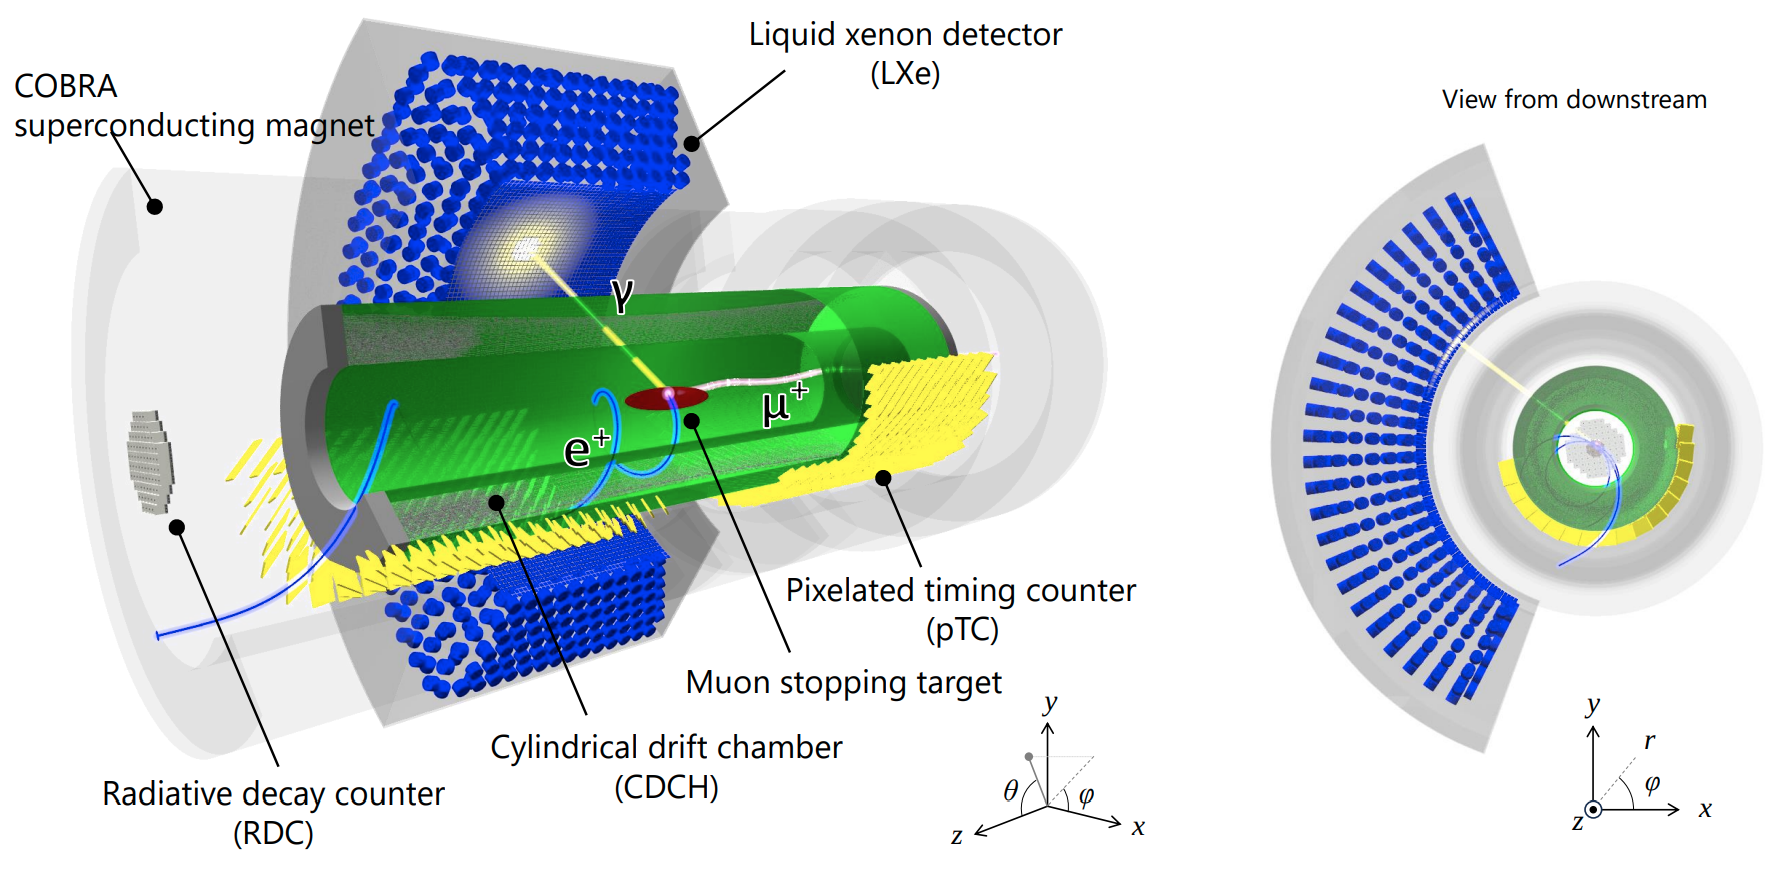
\includegraphics[width =0.8\textwidth]{figures/png/Screenshot_20240307_140116.png}
    \caption{A sketch of the MEG II detector with a simulated $\mu^+ \rightarrow e^+ \gamma $ event, Ref. \cite{megiicollaboration2024operation}.}
    \label{fig:meg22}
    \end{figure}
\begin{figure}[!h]
\centering
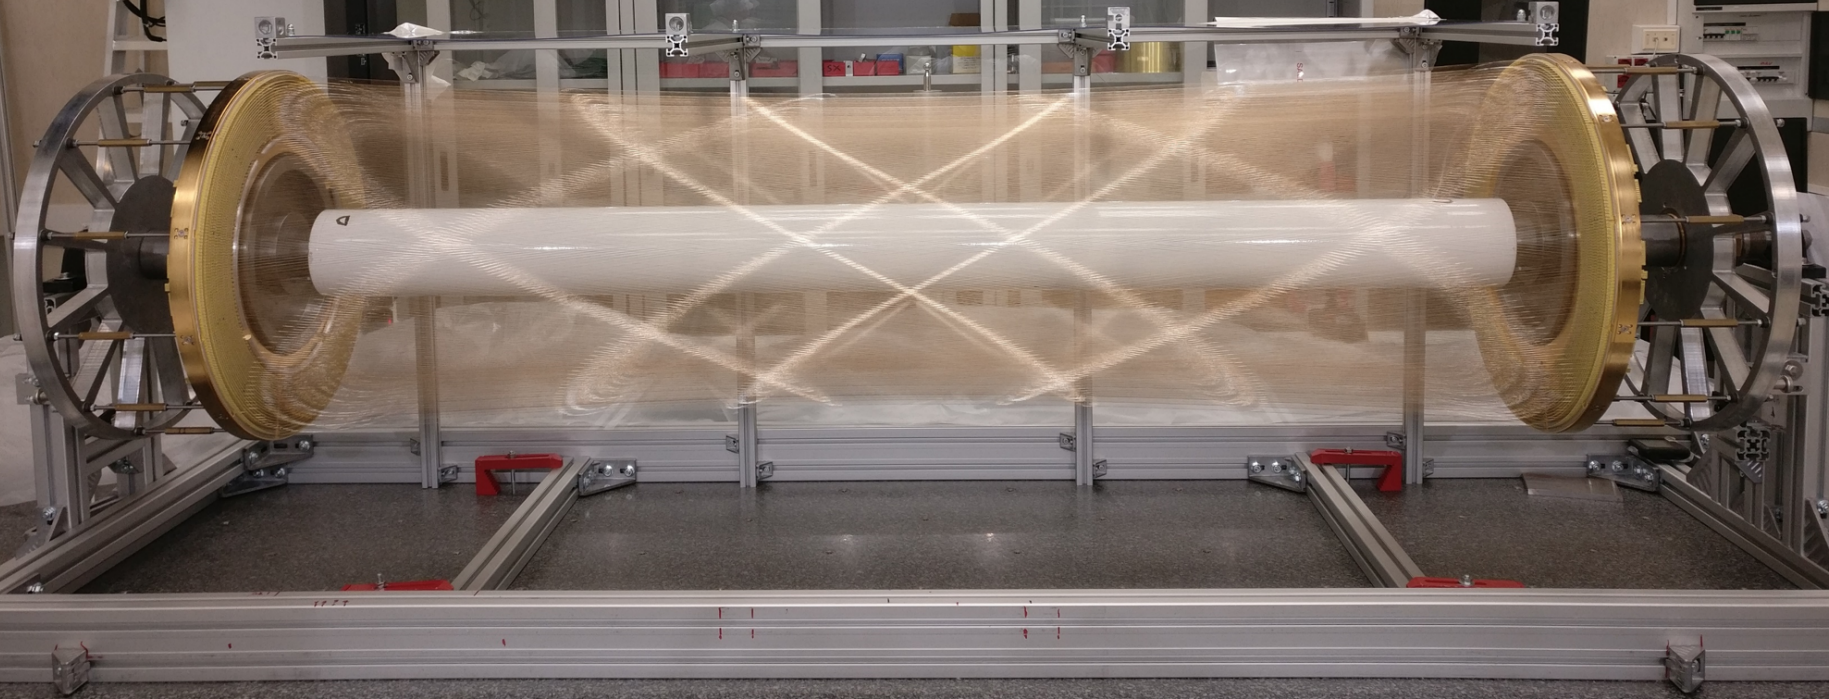
\includegraphics[width =0.8\textwidth]{figures/png/Screenshot_20240307_140235.png}
\caption{Picture of the open CDCH equipped with all the wires, Ref. \cite{megiicollaboration2024operation}.}
\label{fig:meg2}
\end{figure}






\subsubsection{$\mu^+ \rightarrow e^+ e^-  e^+ $}
The CLFV signature of the $\mu^+$ decay at rest consists of two $e^+$ and one $e^-$ at the same time, 
with total energy equal to the muon mass and null vector sum of the
particle momenta.  The exact energy distribution of daughter particles needs understanding of the underlying physics, 
which is currently unknown. To establish detector efficiency, the fraction of particles with momentum over a certain 
threshold requires some physical assumptions.
There are two main sources of background. The first one is the radiative muon decay with 
internal conversion, $\mu^+ \rightarrow e^+ \gamma \nu_e \bar{\nu}_\mu$ with the radiative
photon internally converting into an electron pair $\mu^+ \rightarrow e^+ e^+ e^- \nu_e \bar{\nu}_\mu$. 
This process has a branching ratio of $BR\sim 3.4 \times 10^{-5}$.
An experimental resolution of $\sim$1 MeV is needed in order to be sensitive to the small energy carried off by the neutrinos. 
The second source of background is due to the coincidence of one Michel decay with a $e^+e^-$ pair (1-MD) or two Michel decays with a single $e^-$ (2-MD). 
In this case, the $e^+e^-$ pair can be produced by Bhabha scattering or photon conversion, while the $e^+$
can be produced by Compton scattering or mis-reconstructed $e^+$ and $e^+e^-$ (with the $e^-$ not reconstructed). 
As a consequence, this source of background depends on the muon rate and
can be suppressed with precise vertex reconstruction, timing and track reconstruction.
As in the previous channel, the use of a continuous beam is preferred.
Since this is a three-body decay and particles momenta span a range between few MeV 
and half the muon mass, a thin and low-mass tracker with an excellent resolution is needed. 
\paragraph{SINDRUM I}
The current best limit on $\mu^+ \rightarrow e^- e^+ e^+$, $1.0 \times 10^{- 12}$ at 90\% C.L., was set by the
SINDRUM I experiment at PSI, Ref. \cite{sindrumi}. A schematic view of the SINDRUM spectrometer is given in Figure \ref{fig:sindrumi}. 
The spectrometer consisted of a double cone-shaped stopping target in the middle of five concentric multi-wire proportional chambers surrounded by an array of plastic
scintillator counters inside a solenoidal magnetic field. Considering a 50 MeV $e^-/e^+$, the detector 
apparatus had a momentum resolution at the level of $\sim$1 MeV, a timing
resolution $\leq$1 ns and a vertex resolution of $\sim$1 cm. The trigger consisted of a charge filter, requiring one negative and two positive particles, within a time window of 7 ns, Ref. \cite{universe8060299}.
\begin{figure}[!h]
\centering
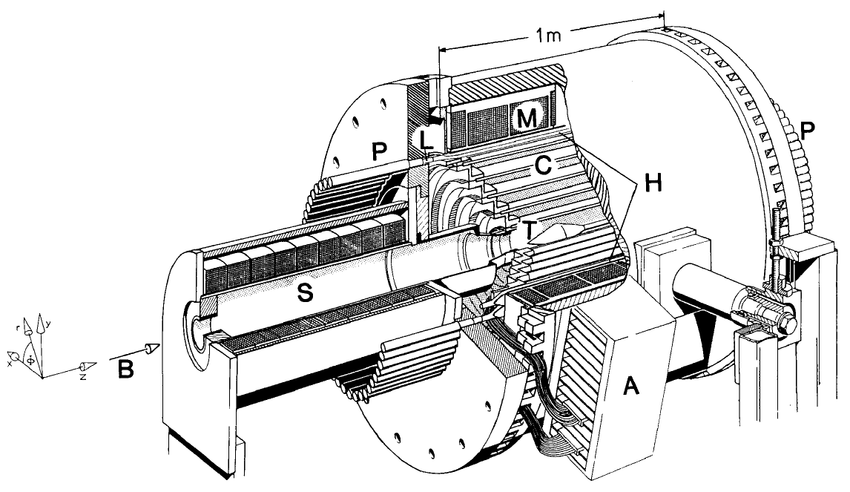
\includegraphics[width =0.8\textwidth]{figures/png/The-SINDRUM-I-detector-in-the-horizontal-operating-orientation.png}
\caption{Schematic view of the SINDRUM experiment, Ref. \cite{sindrumi}.}
\label{fig:sindrumi}
\end{figure}

\paragraph{The Mu3e Experiment}
The goal of the Mu3e experiment is to achieve a single-event-sensitivity of the order
of $10^{-16}$ on the $\mu^+ \rightarrow e^+ e^-  e^+ $ decay, Ref. \cite{hesketh2022mu3e} and \cite{papa}. 
In Figure \ref{fig:mu3e}, a schematic view of Mu3e is shown.
The same muon beam as MEG II experiment will employed, stopping muons on a thin hollow double-come Mylar target. 
A 2 m cylinder will be placed inside a 1.5 T magnetic field and segmented in 5 sections. 
The central station will consist of two double layers of pixel detectors and a
scintillating fiber tracker. The other four stations will be made of two layers of pixel
sensors and a hodoscope of scintillator. Since the Mu3e search relies heavily on accurate track reconstruction, multiple Coulomb
scattering is a limiting factor and the technical choices adopted for the detector design
have been taken to minimize this effect. The tracker consists of High Voltage Monolithic
Active Pixel (HV-MAPS) and the design is such as to exploit the (partial) canceling of
the multiple scattering in half of turn. The estimated time and vertex resolutions are
$\sigma_t \sim 100$ ps and $\sigma_{xy} \sim 200 \ \mu$m and the momentum resolution will be 100 $\div$ 400 keV for 10 $\div$ 53
MeV particles. The experiment is projected in three phases. During the first one, the beam will have an intensity of $\mathcal{O}(10^7) \ \mu^+$/s 
and there will be only the tracker installed. After that, the beam with an intensity of $\mathcal{O}(10^8) \ \mu^+$/s will 
be used and the scintillating fibers and two of the additional tracking stations will be added.
During the third phase, beam intensity will increase up to $\mathcal{0}(10^9) \ \mu^+$/s and to 
reach the single-event-sensitivity of $10^{-16}$, two stations will be added.
\begin{figure}[!h]
\centering
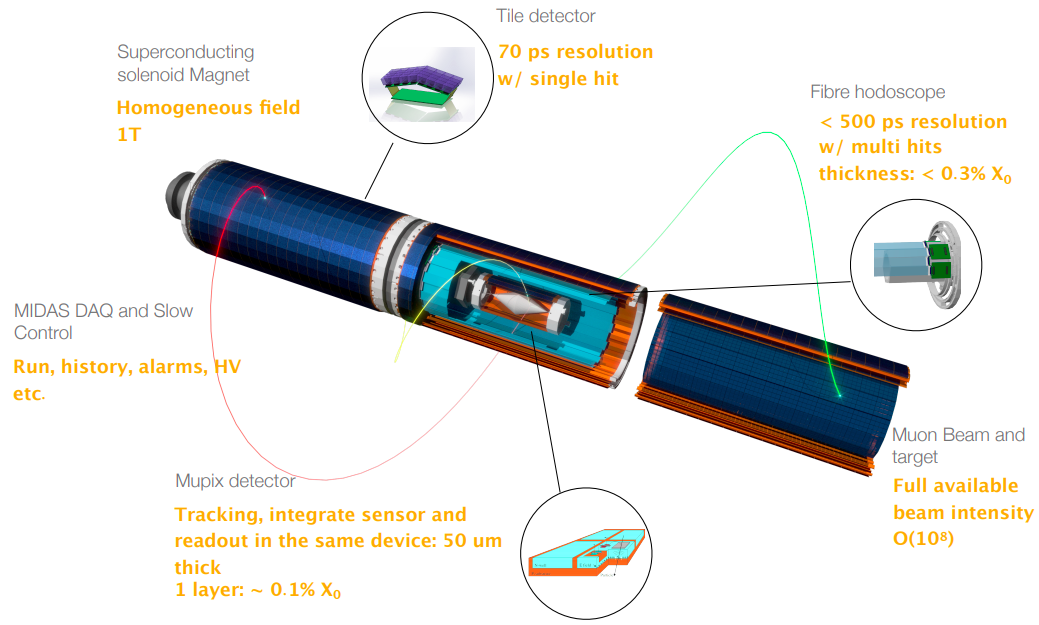
\includegraphics[width =0.8\textwidth]{figures/png/Screenshot_20240321_143650}
\caption{Mu3e experimental setup layout (3D view). An example of a $\mu^+ \rightarrow e^+ e^-  e^+ $ decay event is shown, Ref. \cite{papa}.}
\label{fig:mu3e}
\end{figure}









\subsubsection{$\mu^- N \rightarrow e^- N $}
In this CLFV channel, negative muons are captured by a nucleus and the decay products are detected. The coherent conversion leaves the nucleus
intact and minimal energy will be transmitted to the nucleus recoil.
The signal signature is a monochromatic 105 MeV $e^-$. All other 105 MeV signals may be a source of background. 
Cosmic rays can generate or can be misidentified as electrons in the signal region.
Decay in orbit (DIO) can contaminate the signal region and High energy photons produced by radiative captures of pions (RPC) and muons (RMC) can convert 
asymmetrically and generate high energy electrons. More detailed discussion about signal and backgrounds will be given in Section \ref{sigandbkg}.
Among the previous processes, this channel offers the most powerful sensitivity. 
Thanks to the one particle final state, this channel is not affected by accidental background.
Another advantage, with respect to the $\mu \rightarrow e \gamma$ search, is the larger momentum
and better separation of the electron signal from the background. The background level, due to low-momentum particles, can be reduced
thanks to the \textit{hollow-cylinder} detectors. The muon capture process is incredibly fast ($\mathcal{O}(10^{-13})$ s) and is characterized by the emission of
an X-ray, that can be detected. To cancel the uncertainty due to the overlap of the nucleus and the muon wave
functions, the commonly used quantity to denote results in this type of searches is:
\begin{equation}
    R_{\mu e}=\frac{N(\mu \rightarrow e)}{N(\text{muon capture})}
\end{equation}
Through the detection of X-ray from muon capture, the denominator can be easily determined.
As discussed in Section \ref{sigandbkg}, a pulsed beam is preferred.
A characteristic of these experiments is that the apparatus lend itself to the additional
search of the process $\mu^- N \rightarrow e^+ N$ which would violate also the leptonic number.
\paragraph{SINDRUM II}
PSI delivered a 1 MW 590 MeV proton beam that was extracted from the ring
cyclotron and directed onto a 40 mm carbon target. The beam line
transported secondary particles ($\pi$, $\mu$, $e$) emitted in the backward direction to the SINDRUM II spectrometer, as
illustrated in Figure \ref{fig:sindrumii}. The structure of the experiment
was cylindrical. The gold target (B), which had a radius of 20 mm, was positioned
in the middle of the cylinder. Two drift chambers (F and G) were adopted to measure
the helical trajectories, with the ionization electrons drifting radially towards the amplification 
regions. The tracker used CO$_2$-isobutane (70\%/30\%) as a drift
gas while the second one He-isobutane (85\%/15\%). Two 3 mm thick plastic scintillator hodoscopes (D) and a 3 cm 
thick plexiglass Cherenkov hodoscope (E) provided trigger and time information. 
The device included two end-cap hodoscopes at opposite ends of the tracking zone to aid in triggering 
and resolving ambiguities during event reconstruction.The number of muons stopped
was monitored observing the characteristic muonic gold X-rays passing through the
superconducting coil of the spectrometer. A Ge(Li) detector was used for this purpose.
SINDRUM II set the limit on the muon conversion at $7 \times 10^{-13}$, Ref. \cite{SINDRUMII:2006dvw}.
\begin{figure}[!h]
\centering
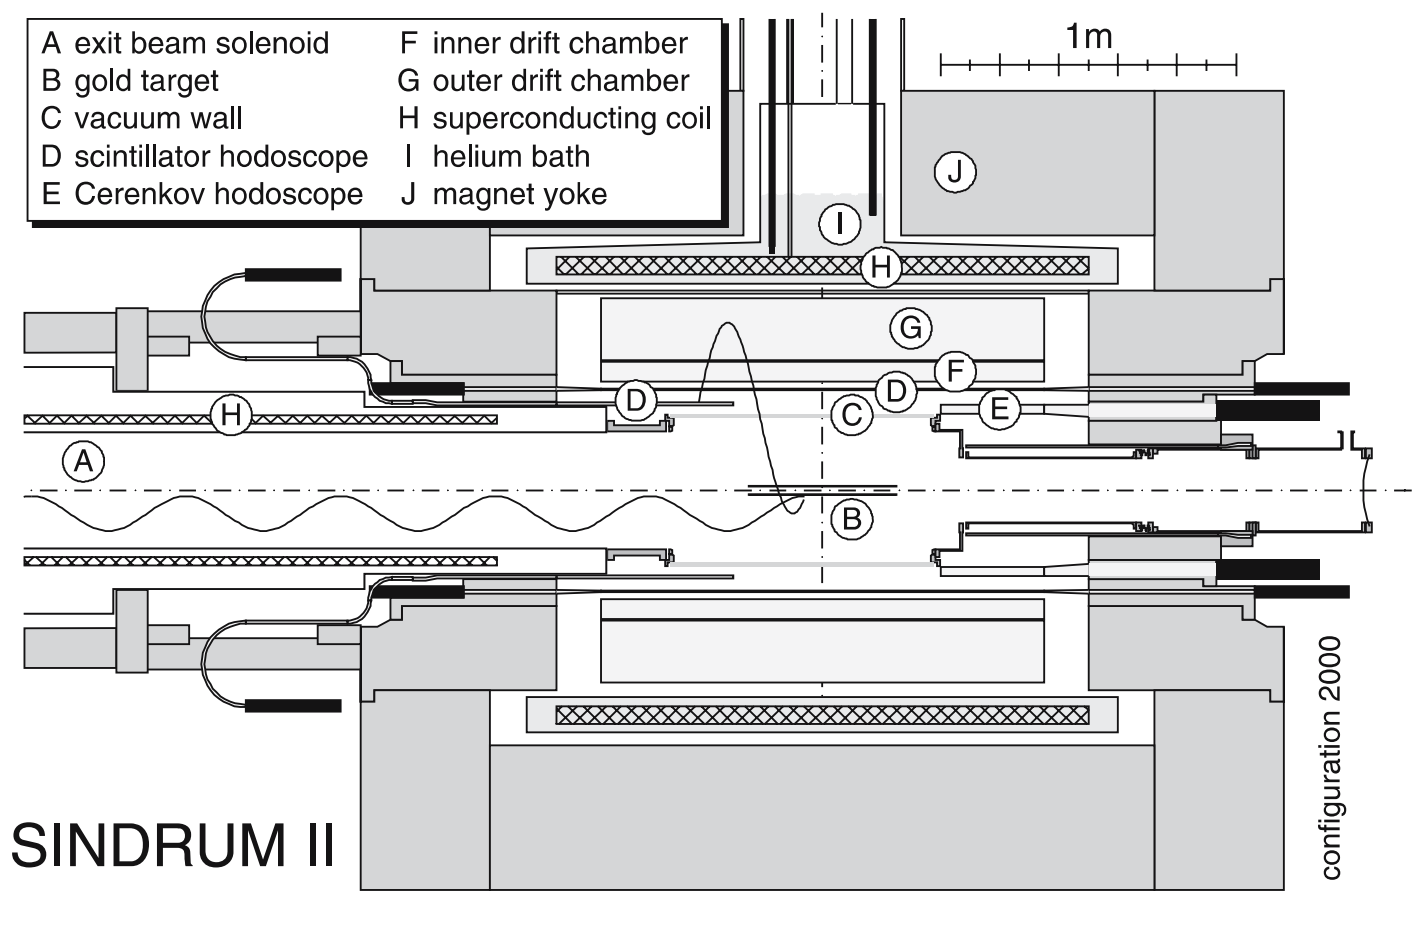
\includegraphics[width =0.8\textwidth]{figures/png/Screenshot_20240307_163120.png}
\caption{Pictorial view of the SINDRUM II experiment, Ref. \cite{SINDRUMII:2006dvw}.}
\label{fig:sindrumii}
\end{figure}
\paragraph{Mu2e}

Mu2e will employ an 8 GeV, 25 kW pulsed proton beam, with 100 ns wide bunches spaced by 1.7 $\mu$s. 
Figure \ref{fig:mu2escheme} shows a schematic view of the experimental setup and of the
three sections of the experiment: Production Solenoid, Transport
Solenoid and Detector Solenoid. The $S$ shape lowers the background due to 
neutral particles and selects the charge sign: almost only negative muons will hit the stopping target. 
The straw tube tracker and the crystal electromagnetic calorimeter are located down-stream of the Al target. 
Both these detectors adopted a \textit{hollow-cylinder} geometry. 
The estimated Mu2e sensitivity after three years of data taking is $R_{\mu e} < 3 \times 10^{-17}$, Ref. \cite{universe9010054}.
Mu2e will be described extensively in the Chapter \ref{mu2echapter}.
The Mu2e Collaboration is also performing preliminary studies for the upgraded Mu2e II, Ref. \cite{dukes}. 
The proton beam intensity will be improved by the PIP-II upgrade that will increase the rate of stopped muons 
on target from $10^{10} \ \mu^-$/s to $10^{11} \ \mu^-$/s. New detector technologies are under study for the upgraded
Mu2e II.
\paragraph{COMET}
The COherent Muon-to-Electron Transition (COMET) experiment is under construction at
the Japanese Proton Accelerator Research Center (J-PARC), Ref. \cite{Abramishvili_2020}. 
This experiment has lots of similarities with Mu2e: COMET will employ a 8 GeV, 56 kW pulsed proton beam
with a separation of 1.17 $\mu$s between the bunches. The two main differences between
COMET and Mu2e can be seen from the schematic view of these experiments.
The presence of a C-shaped (not S-shaped) transport solenoid will allow a tighter
muon momentum selection, traded with a reduced beam intensity $\sim$70\%
An extra curved solenoid after the stopping target will remove most of the non
interesting electrons before reaching the tracker.
COMET will be developed in two stages: Phase-I and Phase-II (Fig. 1.14).

\begin{figure}[!h]
\centering
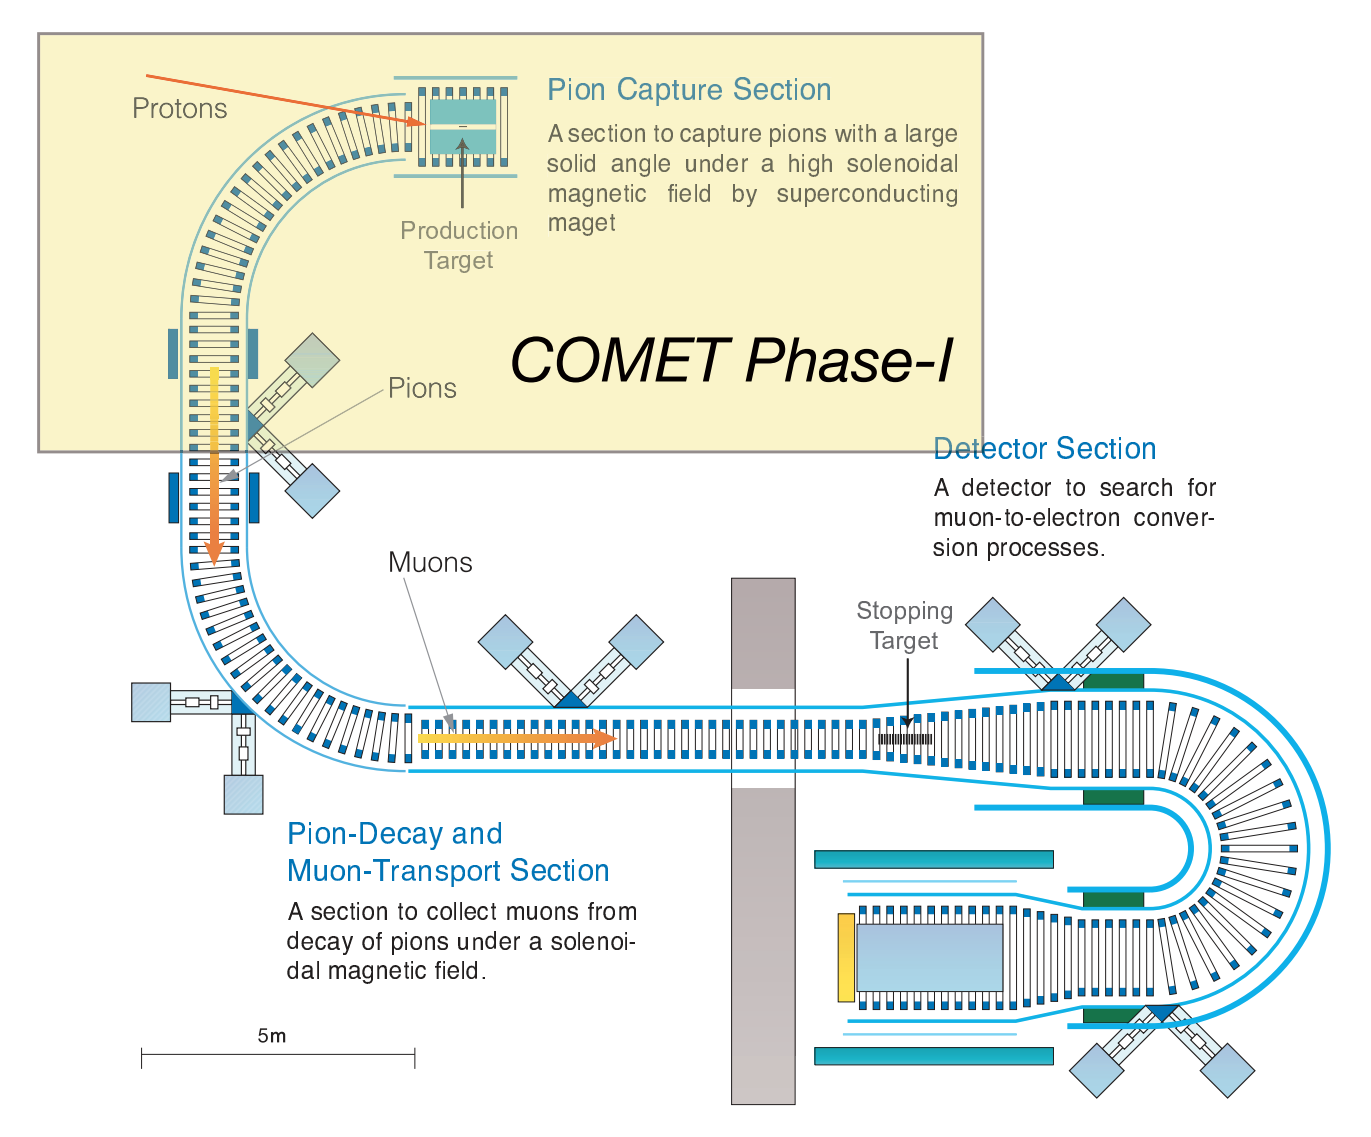
\includegraphics[width =0.4\textwidth]{figures/png/Screenshot_20240307_152133.png}
\caption{Schematic layout of COMET (Phase-II) and COMET Phase-I (not in scale).}
\label{fig:comet}
\end{figure}
\paragraph{DeeMe}
\cite{dukes}
\subsection{$\tau$ Channels}
The $\tau$ lepton is a very promising source of CLFV decays, Ref. \cite{universe8060299}. 
The huge $\tau$ mass ($m_\tau$ $\sim$ 1.777 GeV) allows for the investigation of multiple CLFV channels, in comparison with muon decays, Ref. \cite{clfv_signorelli}: 
$\tau^\pm \rightarrow l^\pm \gamma$, $\tau \rightarrow 3l$ and $\tau\rightarrow l \ h$, 
where $h$ is a light hadron and $l$ is an electron or muon. The $\tau$ sector of a CLFV search takes advantage from an higher predicted branching ratio, compared to muons, 
according to $(\frac{m_\tau}{m_\mu})^\alpha$, where $\alpha$ depends on the model. Table \ref{tab:upperlimits} lists the current best limits on the $\tau$ 
CLFV searches and Figure \ref{fig:tauchannel} displays the results from the BaBar, Ref. \cite{PhysRevD.77.091104}, Belle, Ref. \cite{ABASHIAN2002117} and LHCb, 
Ref. \cite{TheLHCbCollaboration2008}, experiments. The $\tau$ particle has a short lifetime ($\tau_\tau \ \sim$ 2.91 $\times$ 10$^{-13}$ s), with respect to the muon.
As a result, it is not possible to produce $\tau$ beams and strong electron or proton accelerators are required to produce $\tau$s with a large generation cross section. 
To constrain the kinematics of decay, large detectors with good particle identification, tracking, calorimetry, and hermeticity are required. 
Because $\tau$ CLFV searches are done with beams and detectors used for a broader physics programme, 
the increased sensitivity derived by its greater mass is partially decreased by the number of $\tau$s that can be detected.
In these experiments, a pair of $\tau^+ \tau^-$ is produced by the decay of $\Upsilon(4s)$ resonance at $\sqrt{s}=10.58$ GeV. The branching ratio of this process is  $90\%$ of 
the one of $b \bar{b}$. One $\tau$ decays via Standard Model (SM) process (tag side), while the signal side is determined based on the specific topology of each channel. 
At $e^+ e^-$ and $pp$ colliders, the $\tau$s are not created at rest. Because of the boost, the decay products could have 
energy of several GeV, posing an experimental challenge of providing wide-range calibrations for detectors (from a few hundred MeV to several GeV), Ref. \cite{universe8060299}.
In a short time, the Belle 2 experiment at Super KEKB will try to increase its limits below $5 \times 10^{-9}$ or $10^{-9}$ for the radiative and three body decays respectively, 
with an integrated luminosity of 50 ab$^{-1}$. The main background, in $\tau \rightarrow l \gamma$ channel only, arises from
$e^+ e^- \rightarrow \mu^+ \mu^- \gamma$ or $e^+ e^- \rightarrow \tau^+ \tau^- \gamma$ where one of the $\tau$s decays via $\tau \rightarrow \nu \bar{\nu}$.
To reduce the background, it is possible to use the $\tau$ polarization or to collect large samples of
$\tau$ leptons at a lower center-of-mass energy, where initial state radiation is negligible in the signal region. This might be the situation in a $\tau$-charm 
factory operating slightly above the $\tau$ production threshold, Ref. \cite{Bennett_2016}.
\begin{figure}[!h]
\centering
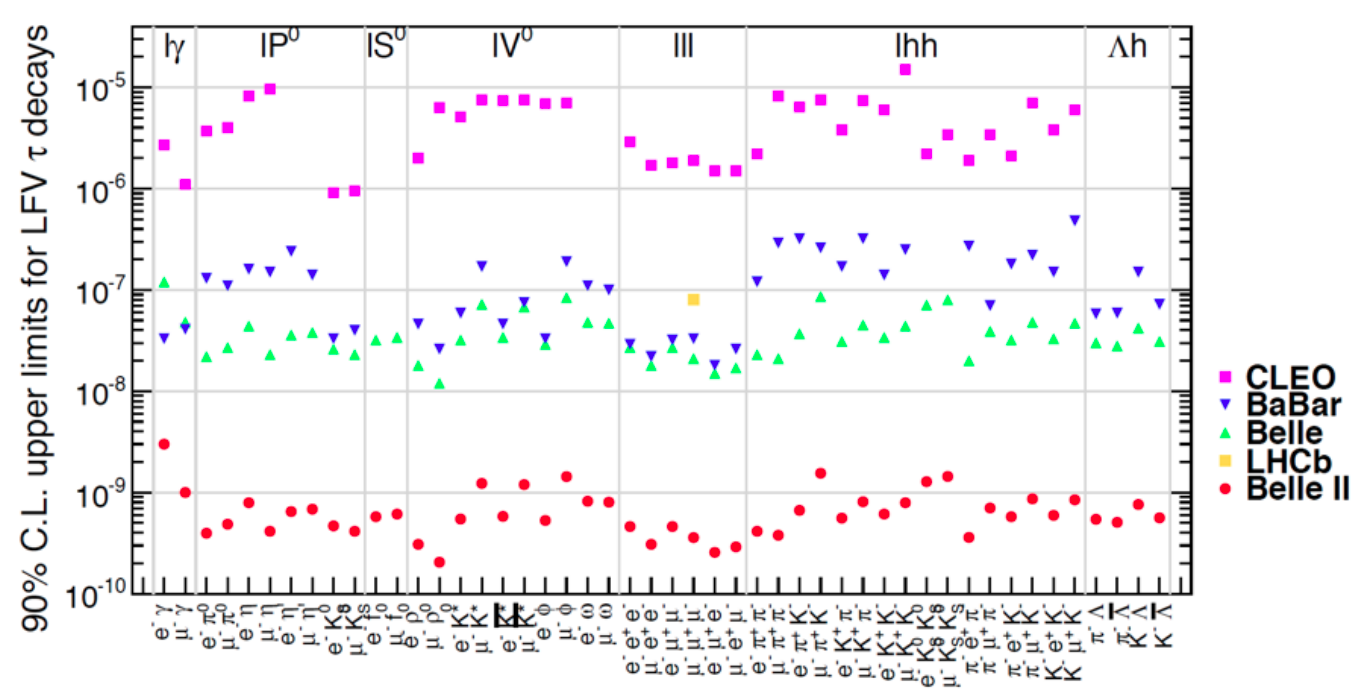
\includegraphics[width =0.8\textwidth]{figures/png/Screenshot_20240319_134052.png}
\caption{Tau lepton-flavor-violating branching ratio 90\% C.L. upper limits summary plot, Ref. \cite{universe4100101}. The green and blue cones 
are respectively the Belle and Babar's best upper limits. The red dots are Belle II's expected upper limits for the 50 ab$^{-1}$ run.}
\label{fig:tauchannel}
\end{figure}

\iffalse
\subsection{$K$ and other Mesons Channels}
There are several CLFV processes that involve $K$ mesons:
\begin{itemize}
    \item Axial Vector and Pseudoscaler: $K^0_L \rightarrow \mu^\pm e^\mp $ and $K^0_L \rightarrow \pi^0 \mu^\pm e^\mp$;
    \item Vector and Scalar: $K^+ \rightarrow \pi^+ \mu^+ e^-$ and $K^+ \rightarrow \pi^+ \mu^- e^+$;
    \item Total lepton number violating: $K^+ \rightarrow \pi^- \mu^+ e^+$.
\end{itemize} 
Kaons have many more decay modes than muons so many more potential sources of background. They also
come with lots of either neutrons and gammas or charged pions.


\begin{figure}[!h]
\centering
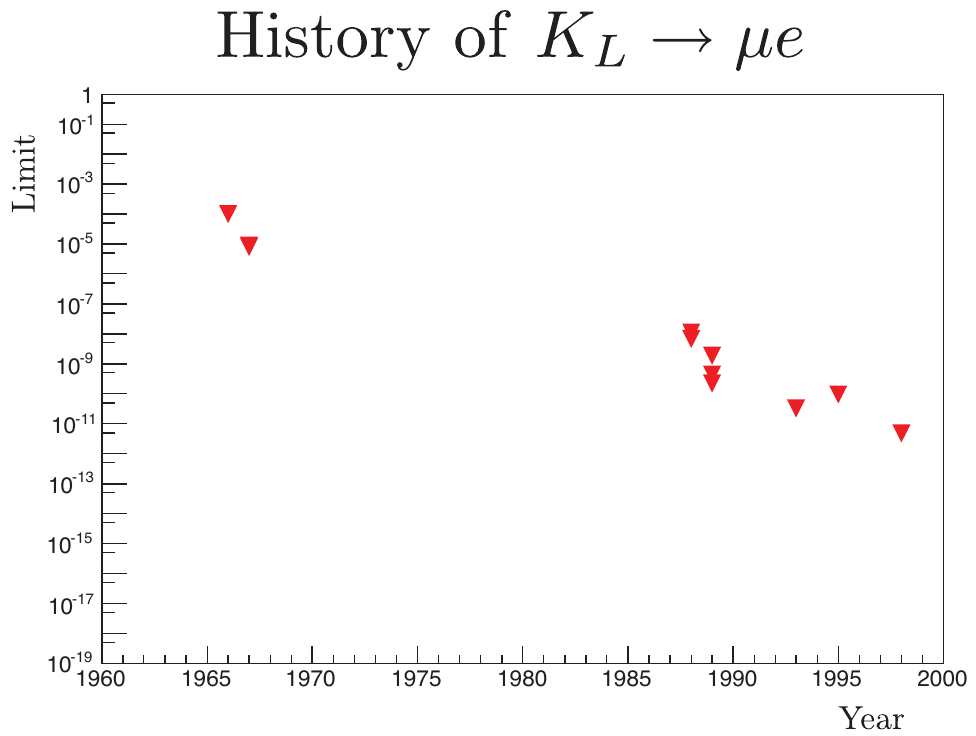
\includegraphics[width =0.4\textwidth]{figures/png/Screenshot_20240307_114258.png}
\caption{.}
\label{fig:Kchannel}
\end{figure}

\fi
